\documentclass[11pt]{article}
\usepackage[a4paper,margin=25mm]{geometry}
\usepackage{mathptmx}
\usepackage[T1]{fontenc}
\usepackage{amsmath,amssymb,amsthm,bm}
\usepackage{graphicx,booktabs,multirow,cite,url,microtype}
\graphicspath{{../../results/fig/}}
\usepackage{float}
\usepackage{algorithm,algorithmic}
\usepackage[hidelinks]{hyperref}
\hypersetup{pdfauthor={Sreeram Anil},pdftitle={A Unified Single-Rigid-Body NMPC/NMHE Framework for ANYmal-C Trotting}}
\usepackage{caption}
\usepackage{tikz}
\usetikzlibrary{positioning}
\captionsetup{font=footnotesize,labelfont=sc,labelsep=period}
\usepackage{titlesec}
\titleformat{\section}{\centering\normalsize\scshape}{\thesection.}{0.5em}{}
\titleformat{\subsection}{\itshape\normalsize}{\thesubsection.}{0.5em}{}
\titleformat{\subsubsection}{\itshape\normalsize}{\thesubsubsection)}{0.5em}{}
\renewcommand{\thesection}{\Roman{section}}
\renewcommand{\thesubsection}{\Alph{subsection}}
\renewcommand{\thesubsubsection}{\arabic{subsubsection}}
\setlength{\parskip}{0pt}\setlength{\parindent}{1em}
\newtheorem{proposition}{Proposition}
\newtheorem{lemma}{Lemma}
\newtheorem{remark}{Remark}
\newtheorem{assumption}{Assumption}
\newcommand{\R}{\mathbb{R}}
\newcommand{\T}{^{\mathsf T}}
\newcommand{\bx}{\bm{x}}\newcommand{\bu}{\bm{u}}\newcommand{\bw}{\bm{w}}\newcommand{\by}{\bm{y}}
\newcommand{\bp}{\bm{p}}\newcommand{\bv}{\bm{v}}\newcommand{\bom}{\bm{\omega}}\newcommand{\bth}{\bm{\theta}}
\newcommand{\bfv}{\bm{f}}\newcommand{\br}{\bm{r}}\newcommand{\bd}{\bm{d}}\newcommand{\bs}{\bm{s}}
\newcommand{\Rot}{\bm{R}}\newcommand{\Tm}{\bm{T}}\newcommand{\I}{\bm{I}}
\newcommand{\sk}[1]{\left[#1\right]_\times}
\newcommand{\norm}[1]{\left\|#1\right\|}

\newcommand{\ie}{i.e.}\newcommand{\eg}{e.g.}
\usepackage{fancyhdr}
\pagestyle{fancy}\fancyhf{}\fancyhead[L]{\footnotesize TECHNICAL REPORT --- UNIFIED SRBD NMPC/NMHE FOR ANYMAL-C}\fancyhead[R]{\footnotesize\thepage}\renewcommand{\headrulewidth}{0pt}

\title{\LARGE A Unified Single-Rigid-Body NMPC/NMHE Framework for\\ ANYmal-C Trotting:\\[2pt] \large Model Derivation, Output-Feedback Architecture, and Closed-Loop MuJoCo Validation}
\author{Sreeram Anil\\[2pt]
\small Technical report, September 2026\\[1pt]
\small Simulation study built around a real-time-iteration NMPC solver and its moving-horizon-estimation variant,\\
\small developed as an extension of the author's master's thesis on SLQP-MPC. The solver algorithms are unpublished\\
\small ongoing research and are not described here; this report covers the modelling, the architecture and the results.}
\date{}

\begin{document}
\maketitle

\begin{abstract}
This report derives and validates a unified output-feedback control architecture for the ANYmal-C quadruped in which a nonlinear model predictive controller (NMPC) and a nonlinear moving-horizon estimator (NMHE) share one single-rigid-body-dynamics (SRBD) model, one symbolic source, and one algorithmic design language. The controller and the estimator are instances of a real-time-iteration NMPC solver and its moving-horizon-estimation variant, developed as an extension of the author's master's thesis on SLQP-MPC; both are used as unmodified libraries behind a small C interface, and their algorithms---ongoing unpublished work---are outside the scope of this report. The two solver-facing interfaces of the SRBD model---time-varying foot positions, contact schedule and disturbance parameters for the controller, and known inputs, measurement gates and an augmented random-walk disturbance state for the estimator---are realised entirely in the generated model header and in a thin driver. We derive the SRBD model in ZYX Euler coordinates with body-frame angular velocity, the gait-scheduled contact parametrisation, the friction-cone and attitude constraints, the leg-odometry and IMU measurement model with settled-stance gating, the augmented-state disturbance observer, and the joint closed loop with disturbance feed-forward. We explain why a disturbance modelled as a penalised estimator input is recovered too slowly for feed-forward and why carrying it as a random-walk state removes the lag. On a MuJoCo full-body simulation of ANYmal-C (18 DoF, 45~kg, 57\,\% of the mass in the legs) the loop performs a trot at 0.4~m/s, absorbs a 40~N lateral push, and executes a 0.3~rad/s turn with a 50-stage, 100~Hz NMPC costing 0.56~ms preparation and 56~$\mu$s feedback per cycle, and a 20-node, 100~Hz NMHE costing 0.24~ms preparation, 1.1~$\mu$s instantaneous output and 37~$\mu$s feedback. Velocity is estimated to 1~cm/s, attitude to 1.4--2.6~mrad, a 60~N push to 61.8~N; force feed-forward of the estimated wrench reduces the push-induced drift from 0.74~m to 0.15~m. Five noise seeds succeed. The modelling, the simulation framework, the data and the animation are released; the solver libraries are not.
\end{abstract}

\section{Introduction}
Legged locomotion is the natural system-level test of a matched control--estimation pair. The controller must select ground reaction forces (GRFs) inside friction cones over a horizon that spans several contact switches, and the estimator must reconstruct the base state from proprioception alone---an IMU and the leg kinematics of whichever feet are on the ground---while the contact set changes every few hundred milliseconds. Both problems are constrained, nonlinear, and must be solved at hundreds of hertz. The reduced-order single-rigid-body model (SRBD) is the standard compromise between fidelity and speed for the controller \cite{dicarlo2018,bledt2018,kim2019}; for the estimator the same rigid-body model is the natural companion, because it makes the estimated quantities exactly the ones the controller consumes.

The solvers used here are a matched pair developed as an extension of the author's master's thesis on SLQP-MPC \cite{thesis}: a real-time-iteration NMPC solver with state constraints, and a moving-horizon estimator with state and input constraints, both in plain C with compile-time dimensions and microsecond-scale cycles \cite{solvers}. That work is ongoing and unpublished, so this report treats both as libraries behind the small interface released with the code \cite{repo}, and says nothing about how they work inside. What it does report is the system-level question they were built for: whether one reduced-order model, instantiated once as a controller and once as an estimator, closes an output-feedback walking loop on a full-body robot, and what the modelling has to get right for that to happen.

\subsection{Contributions}
\begin{enumerate}
\item A complete derivation of the ANYmal-C SRBD model, gait parametrisation, constraints, costs and proprioceptive measurement model, generated from one SymPy source and instantiated once for the controller (Sec.~IV) and once for the estimator (Sec.~V).
\item Two integration mechanisms that keep both solver libraries unmodified: an out-of-band stage-parameter table for the NMPC, and a known-input encoding of the contact schedule, foot anchors and measurement gates for the NMHE (Sec.~IV-B, V-B).
\item An account of why a disturbance modelled as a penalised estimator input cannot be fed forward in a single-iteration setting, and its removal by an augmented random-walk disturbance state (Sec.~V-A).
\item A leg-odometry measurement model with contact detection, settled-stance gating and contact-point Jacobians whose necessity is demonstrated by ablation during development (Sec.~III-F).
\item A closed-loop validation on the full-body MuJoCo model with sensor noise, a lateral push and a turn, with timing, accuracy, ablation and noise-sensitivity data, an animation, and a released simulation framework (Sec.~VII--VIII).
\end{enumerate}

\subsection{Scope and honesty statement}
The SRBD is a deliberately coarse model of a robot whose legs carry 57\,\% of the mass. The report documents what this costs (touchdown residuals, a 5--10\,\% forward-speed deficit, torque-channel feed-forward that must stay open-loop) as carefully as what it buys. No third-party optimality oracle (IPOPT) was available in the build environment, so the quality of the solutions is established by the solver's own fixed-parameter convergence to a $10^{-10}$ KKT residual and by the agreement of its two linearisation modes, not by an external solve. The solver algorithms are deliberately absent: what is reported about them is only what a user of the interface can measure, namely per-cycle wall times, memory footprint and horizon scaling.

\subsection{Notation}
Vectors are bold; $\sk{\bm a}$ is the cross-product matrix; $\bm e_j$ the $j$-th unit vector; $c_\alpha,s_\alpha,t_\alpha$ are $\cos,\sin,\tan$; $\|\bm a\|^2_Q=\bm a\T Q\bm a$; $\succeq$ denotes positive semidefiniteness. Subscript $k$ is a stage/node index, $t$ a sampling instant, $i$ a leg. Table~\ref{tab:notation} collects the symbols.
\begin{table}[t]\centering\caption{Symbols.}\label{tab:notation}
\footnotesize\begin{tabular}{@{}ll@{}}\toprule
$\bp,\bv$ & system-COM position/velocity, world frame\\
$\bth=(\phi,\theta,\psi)$, $\Rot$, $\Tm$ & ZYX Euler angles, rotation $\mathcal B\to\mathcal W$, Euler-rate map\\
$\bom$ & angular velocity, body frame\\
$\bfv_i,\br_i,s_i$ & GRF, contact point, contact flag of leg $i$\\
$\bd=(\bd_f,\bd_\tau)$ & disturbance wrench (world force, body torque)\\
$\bw$ & estimated input of the NMHE ($=\dot\bd$)\\
$\pi_k=(\br_k,\bs_k,\bd)$ & NMPC stage parameters\\
$\bu_k$ & NMHE known input \eqref{eq:uk}\\
$s^m_i,g_v,\delta_i$ & measurement gates, velocity gate, contact detection\\
$m,\I,\mu,f_{\max}$ & mass, inertia, friction coefficient, force bound\\
$N,M,h$ & NMPC horizon, NMHE window, sampling period\\
$Q,R,Q_N$; $V,W,\Lambda_a$ & NMPC weights; NMHE weights and arrival information\\

$T_g,\beta,\varphi_i,\sigma_i$ & gait period, duty factor, leg phase, swing phase\\
\bottomrule\end{tabular}\end{table}

\section{Related Work}
\textbf{SRBD MPC for quadrupeds.} Di Carlo et al.\ \cite{dicarlo2018} introduced convex MPC on a linearised SRBD with gait-scheduled contacts and Raibert-style footholds for the MIT Cheetah~3; Bledt et al.\ \cite{bledt2018} and Kim et al.\ \cite{kim2019} combined it with whole-body control. Nonlinear SRBD MPC solved by SQP/RTI appears in \cite{farshidian2017,grandia2019} on ANYmal with the OCS2 toolbox, and the SLQ/DDP family \cite{farshidian2017} remains the workhorse for kino-dynamic models. Our controller is a nonlinear SRBD MPC in the sense of \cite{grandia2019}, with hard friction cones and attitude bounds handled inside the solver rather than by a separate QP.

\textbf{Legged state estimation.} Bloesch et al.\ \cite{bloesch2013} established the leg-odometry EKF that fuses IMU with kinematic foot constraints, treating foot positions as states; Camurri et al.\ \cite{camurri2020} and Wisth et al.\ \cite{wisth2019} extended this to factor graphs; moving-horizon formulations for legged systems have been explored more recently as solver speed has made them affordable. Our estimator follows the leg-odometry principle but replaces the EKF by a constrained moving-horizon estimator on the same SRBD the controller uses, with a random-walk wrench state in the spirit of disturbance observers for offset-free MPC \cite{pannocchia2003}.

\textbf{Solvers.} The real-time-iteration idea---one Newton-type iteration per sampling instant, split into a preparation phase and a feedback phase---goes back to Diehl et al.\ \cite{diehl2005} and is the operating mode assumed throughout this report; \texttt{acados} \cite{acados} is the reference open-source implementation and is a drop-in substitute behind the interface used here. The particular solvers used in this study are the author's own \cite{solvers,thesis}; their formulation and numerics are unpublished and are not part of this report.

\section{System Model}
\subsection{Frames and attitude parametrisation}
Let $\mathcal W$ be the inertial (world) frame with $z$ up and $\mathcal B$ the base frame of ANYmal-C with $x$ forward, $y$ left, $z$ up. The SRBD state is
\begin{equation}
\bx=\begin{bmatrix}\bp\\ \bth\\ \bv\\ \bom\end{bmatrix}\in\R^{12},\qquad
\begin{aligned}
&\bp\in\R^3 &&\text{COM position in }\mathcal W,\\
&\bth=(\phi,\theta,\psi) &&\text{roll, pitch, yaw (ZYX)},\\
&\bv\in\R^3 &&\text{COM velocity in }\mathcal W,\\
&\bom\in\R^3 &&\text{angular velocity in }\mathcal B.
\end{aligned}
\label{eq:state}
\end{equation}
The rotation from $\mathcal B$ to $\mathcal W$ is
\begin{equation}
\Rot(\bth)=\Rot_z(\psi)\Rot_y(\theta)\Rot_x(\phi),
\label{eq:R}
\end{equation}
with the elementary rotations $\Rot_x(\phi)=\left[\begin{smallmatrix}1&0&0\\0&c_\phi&-s_\phi\\0&s_\phi&c_\phi\end{smallmatrix}\right]$, $\Rot_y(\theta)=\left[\begin{smallmatrix}c_\theta&0&s_\theta\\0&1&0\\-s_\theta&0&c_\theta\end{smallmatrix}\right]$, $\Rot_z(\psi)=\left[\begin{smallmatrix}c_\psi&-s_\psi&0\\s_\psi&c_\psi&0\\0&0&1\end{smallmatrix}\right]$. Positive pitch is nose-down. The body angular velocity relates to the Euler rates through
\begin{equation}
\dot{\bth}=\Tm(\bth)\,\bom,\qquad
\Tm(\bth)=\begin{bmatrix}1 & s_\phi t_\theta & c_\phi t_\theta\\ 0 & c_\phi & -s_\phi\\ 0 & s_\phi/c_\theta & c_\phi/c_\theta\end{bmatrix},
\label{eq:T}
\end{equation}
where $t_\theta=\tan\theta$; $\Tm$ is singular only at $\theta=\pm\pi/2$, far outside the attitude bounds enforced by both the controller and the estimator (Sec.~IV-A, V-B). The world-frame angular velocity is $\Rot\bom$; we keep $\bom$ in $\mathcal B$ because that is what a body-mounted gyroscope measures and because the inertia tensor is then constant.

\subsubsection{Derivation of the Euler-rate map}
Differentiating \eqref{eq:R} and using $\dot\Rot=\Rot\sk{\bom}$ (definition of the body angular velocity) gives $\sk{\bom}=\Rot\T\dot\Rot$. Each factor contributes an elementary rotation about its own axis, $\dot\Rot_x(\phi)=\Rot_x\sk{\dot\phi\,\bm e_1}$ etc., so that
\begin{align*}
\sk{\bom}&=\Rot_x\T\Rot_y\T\big(\dot\psi\sk{\bm e_3}\big)\Rot_y\Rot_x\\&\quad+\Rot_x\T\big(\dot\theta\sk{\bm e_2}\big)\Rot_x+\dot\phi\sk{\bm e_1},
\end{align*}
and with $\Rot\T\sk{\bm a}\Rot=\sk{\Rot\T\bm a}$,
\begin{equation}
\bom=\dot\phi\,\bm e_1+\dot\theta\,\Rot_x\T\bm e_2+\dot\psi\,\Rot_x\T\Rot_y\T\bm e_3
=\begin{bmatrix}1&0&-s_\theta\\0&c_\phi&s_\phi c_\theta\\0&-s_\phi&c_\phi c_\theta\end{bmatrix}\dot\bth=:\bm E(\bth)\dot\bth.
\label{eq:E}
\end{equation}
$\bm E$ has determinant $c_\theta$; its inverse is $\Tm=\bm E^{-1}$ in \eqref{eq:T}, singular at $\theta=\pm\pi/2$. The derivatives $\partial(\Tm\bom)/\partial\phi$ and $\partial(\Tm\bom)/\partial\theta$ that enter $A_k$ (Appendix~A) follow from $\partial\Tm=-\Tm(\partial\bm E)\Tm$.

\subsection{Single-rigid-body dynamics}
Let $m$ be the total robot mass and $\I\in\R^{3\times3}$ the composite inertia about the COM expressed in $\mathcal B$, evaluated once in the nominal stance (Sec.~III-G). Leg $i\in\{\mathrm{LF},\mathrm{RF},\mathrm{LH},\mathrm{RH}\}$ ($i=1,\dots,4$) applies a world-frame ground reaction force $\bfv_i\in\R^3$ at the foot contact point $\br_i\in\R^3$ (world frame) when its contact flag $s_i\in\{0,1\}$ is one. A world-frame disturbance force $\bd_f$ and a body-frame disturbance torque $\bd_\tau$ collect everything the SRBD does not model (leg inertia, external pushes, model error). The Newton--Euler equations of the lumped body are
\begin{subequations}\label{eq:srbd}
\begin{align}
\dot\bp &= \bv,\\
\dot\bth &= \Tm(\bth)\,\bom,\\
m\,\dot\bv &= \sum_{i=1}^4 s_i\bfv_i + m\bm g + \bd_f,\\
\I\,\dot\bom &= \Rot(\bth)\T\sum_{i=1}^4 s_i\,\sk{\br_i-\bp}\bfv_i - \sk{\bom}\I\bom + \bd_\tau,
\end{align}
\end{subequations}
with $\bm g=(0,0,-9.81)$ and $\sk{\bm a}$ the cross-product matrix. Equation \eqref{eq:srbd} is written once and reused by both solvers, with $\bd=(\bd_f,\bd_\tau)$ playing the role of a known stage parameter in the controller (Sec.~IV) and of an estimated augmented state in the estimator (Sec.~V). We write \eqref{eq:srbd} compactly as
\begin{equation}
\dot\bx = f_c(\bx,\bfv;\br,\bs,\bd),\qquad \bfv=(\bfv_1,\dots,\bfv_4)\in\R^{12}.
\label{eq:fc}
\end{equation}
Two conventions matter for what follows. (i) The forces are multiplied by the flags $s_i$ \emph{inside the dynamics} rather than being removed from the decision vector: the controller's input dimension stays fixed at $n_u=12$ across the gait, swing-leg forces are simply decoupled from the dynamics and driven to zero by the cost and the cone $f_{i,z}\ge0$, and the constraint set never changes dimension---which is what a solver with compile-time fixed shapes requires. (ii) The moment arm $\br_i-\bp$ uses the COM, not the base origin; the COM offset of the leg configuration is part of the kinematic measurement model (Sec.~III-F).

\subsubsection{Origin of the lumped model and meaning of the disturbance wrench}
For the full multibody system with bodies $b$ of mass $m_b$, COM positions $\bp_b$ and total mass $m=\sum_b m_b$, Newton's law for the system COM $\bp=\frac1m\sum_b m_b\bp_b$ is exact,
\begin{equation}
m\ddot\bp=\sum_i\bfv_i+m\bm g+\bm F_{\mathrm{ext}},
\label{eq:newton_exact}
\end{equation}
because joint forces are internal. Likewise the angular momentum about the COM, $\bm L=\sum_b\big(m_b\sk{\bp_b-\bp}\dot\bp_b+\Rot_b\I_b\Rot_b\T\bom^{\mathcal W}_b\big)$, obeys exactly
\begin{equation}
\dot{\bm L}=\sum_i\sk{\br_i-\bp}\bfv_i+\bm\tau_{\mathrm{ext}}.
\label{eq:euler_exact}
\end{equation}
The SRBD approximates $\bm L\approx\Rot\I\bom$ with $\I$ the composite inertia of the nominal configuration, \ie\ it neglects (a) the momentum of the legs relative to the trunk and (b) the configuration dependence of $\I$. Differentiating with $\dot\Rot=\Rot\sk{\bom}$ gives $\dot{\bm L}\approx\Rot(\I\dot\bom+\sk{\bom}\I\bom)$, and \eqref{eq:euler_exact} becomes the last row of \eqref{eq:srbd} after left-multiplication by $\Rot\T$. The quantities dropped in (a)--(b) are exactly what the disturbance wrench absorbs:
\begin{equation}
\bd_f=\bm F_{\mathrm{ext}},\qquad
\bd_\tau=\Rot\T\bm\tau_{\mathrm{ext}}+\Rot\T\big(\Rot(\I\dot\bom+\sk{\bom}\I\bom)-\dot{\bm L}\big),
\label{eq:dmeaning}
\end{equation}
which makes the estimated $\hat\bd_\tau$ in Fig.~\ref{fig:dist} interpretable: its gait-frequency component is the reaction of the swinging legs and the configuration dependence of the inertia, its mean the external torque. For the force channel the approximation is exact ($\bd_f$ is only the external force), which is why force feed-forward is safe and torque feed-forward is not (Sec.~VI). The velocity $\bv$ in \eqref{eq:state} is the velocity of the \emph{system} COM, consistent with \eqref{eq:newton_exact}; this is why the measurement model \eqref{eq:vkin} carries a relative COM-velocity term.

\subsection{Discrete-time model}
Both solvers integrate \eqref{eq:fc} with their own explicit RK4 step over the sampling period $h$ (10~ms) with one substep,
\begin{equation}
\bx_{k+1}=F(\bx_k,\bfv_k;\pi_k)=\bx_k+\tfrac{h}{6}(k_1+2k_2+2k_3+k_4),
\label{eq:rk4}
\end{equation}
where $\pi_k=(\br_k,\bs_k,\bd_k)$ is the stage parameter and $k_1,\dots,k_4$ the usual RK4 slopes evaluated with $\pi_k$ frozen over the step. The sensitivities $A_k=\partial F/\partial\bx$ and $B_k=\partial F/\partial\bfv$ are assembled by the solvers' chain rule from the continuous Jacobians $\partial f_c/\partial\bx$ and $\partial f_c/\partial\bfv$, which are generated symbolically with common-subexpression elimination (Appendix~A gives their structure). Contact flags are held constant inside a step; a contact switch is therefore aligned to the 10~ms grid, which is the resolution of the gait scheduler anyway.

Writing $J_x=\partial f_c/\partial\bx$ and $J_u=\partial f_c/\partial\bfv$ at the four RK4 evaluation points $\bx^{(1)}=\bx_k$, $\bx^{(2)}=\bx_k+\tfrac h2k_1$, $\bx^{(3)}=\bx_k+\tfrac h2k_2$, $\bx^{(4)}=\bx_k+hk_3$ (superscripts on $J$ below), the exact discrete sensitivities are the forward-mode chain rule of \eqref{eq:rk4},
\begin{equation}
\begin{aligned}
K^x_1&=J_x^{(1)},\quad K^x_2=J_x^{(2)}(I+\tfrac h2K^x_1),\\
K^x_3&=J_x^{(3)}(I+\tfrac h2K^x_2),\quad K^x_4=J_x^{(4)}(I+hK^x_3),\\
K^u_1&=J_u^{(1)},\quad K^u_2=J_u^{(2)}+\tfrac h2J_x^{(2)}K^u_1,\\
K^u_3&=J_u^{(3)}+\tfrac h2J_x^{(3)}K^u_2,\quad K^u_4=J_u^{(4)}+hJ_x^{(4)}K^u_3,\\
A_k&=I+\tfrac h6\big(K^x_1+2K^x_2+2K^x_3+K^x_4\big),\\
B_k&=\tfrac h6\big(K^u_1+2K^u_2+2K^u_3+K^u_4\big),
\end{aligned}
\label{eq:rk4sens}
\end{equation}
which is what both solver libraries compute from the generated model. Per stage the SRBD costs four evaluations of $f_c$, $J_x$ ($12\times12$) and $J_u$ ($12\times12$) plus six $12\times12\times12$ products. The verification of Sec.~VII-A checks \eqref{eq:rk4sens} against central differences of the discrete map.

\subsection{Gait scheduling and contact parametrisation}
A trot is a periodic schedule with period $T_g$ and duty factor $\beta$ (stance fraction). With per-leg phase offsets $o=(0,\tfrac12,\tfrac12,0)$ for (LF, RF, LH, RH), leg $i$ has phase and contact flag
\begin{equation}
\varphi_i(t)=\Big(\frac{t-t_0}{T_g}+o_i\Big)\bmod 1,\qquad s_i(t)=\mathbb 1[\varphi_i(t)<\beta],
\label{eq:gait}
\end{equation}
so that the diagonal pairs (LF,RH) and (RF,LH) alternate. Before $t_0$ the robot stands ($s\equiv1$). We use $T_g=0.7$~s and $\beta=0.5$ (0.35~s stance, 0.35~s swing); $T_g=0.5$--$0.6$~s produced markedly larger roll excursions on this robot (Sec.~VIII-E). The within-swing phase is $\sigma_i=(\varphi_i-\beta)/(1-\beta)\in[0,1]$ and the next touchdown time of a swinging leg is $t_{\mathrm{td},i}=t+(1-\varphi_i)T_g$.

\subsubsection{Footholds (Raibert heuristic)}
Let $\bm\ell_i\in\R^2$ be the nominal horizontal offset of foot $i$ from the COM in $\mathcal B$ (from the nominal stance, $\pm0.45$~m longitudinally and $\pm0.30$~m laterally). For a leg that touches down at $t_{\mathrm{td}}$, the target is
\begin{equation}
\begin{aligned}
\br_i^{\mathrm{td}} &= \bp + \bv(t_{\mathrm{td}}-t) + \Rot_z(\psi_{\mathrm{td}})\begin{bmatrix}\bm\ell_i\\0\end{bmatrix}
+ \tfrac12 T_{\mathrm{st}}\,\bv + k_r(\bv-\bv^{\mathrm{cmd}}),\\
\psi_{\mathrm{td}} &= \psi+\omega^{\mathrm{cmd}}_z(t_{\mathrm{td}}-t),\qquad r^{\mathrm{td}}_{i,z}=z_{\mathrm{ground}},
\end{aligned}
\label{eq:raibert}
\end{equation}
with $T_{\mathrm{st}}=\beta T_g$ the stance duration and $k_r=0.12$~s a capture-point-like gain (the linear inverted pendulum gives $\sqrt{z/g}\approx0.21$~s; smaller values proved sufficient and calmer). The neutral point $\tfrac12T_{\mathrm{st}}\bv$ uses the \emph{actual} velocity: using the commanded velocity places the foot ahead of the sweep whenever the robot is slower than commanded and brakes it (Sec.~VIII-E). $\bv^{\mathrm{cmd}}=\Rot_z(\psi_{\mathrm{td}})\bv^{\mathrm{cmd}}_{\mathcal B}$ rotates the body-frame command into $\mathcal W$; $z_{\mathrm{ground}}$ is the mean height of the currently anchored stance feet (Sec.~III-F). All quantities in \eqref{eq:raibert} are evaluated with the \emph{estimated} state.

\subsubsection{Swing-foot trajectory}
For $\sigma\in[0,1]$ the desired contact-point position and velocity are
\begin{equation}
\begin{aligned}
\bp^{\mathrm{sw}}_i(\sigma)&=\bp^{\mathrm{lo}}_i+(\br^{\mathrm{td}}_i-\bp^{\mathrm{lo}}_i)\,\varsigma(\sigma)
+\begin{bmatrix}0\\0\\ h_{\mathrm{sw}}\,\beta_4(\sigma)+z_{\mathrm{land}}\,\varsigma(\sigma)\end{bmatrix},\\
\varsigma(\sigma)&=10\sigma^3-15\sigma^4+6\sigma^5,\qquad \beta_4(\sigma)=16\sigma^2(1-\sigma)^2,
\end{aligned}
\label{eq:swing}
\end{equation}
where $\bp^{\mathrm{lo}}_i$ is the lift-off position, $h_{\mathrm{sw}}=0.06$~m the apex height and $z_{\mathrm{land}}=-0.015$~m a deliberate overshoot below the ground so that contact is established slightly \emph{before} the scheduled touchdown. Both $\varsigma$ and $\beta_4$ have zero velocity at $\sigma=0,1$; a $\sin(\pi\sigma)$ height profile, whose end slope is $-\pi h_{\mathrm{sw}}/T_{\mathrm{sw}}\approx-0.5$~m/s, produced 540--590~N impacts against 290--310~N commands and was replaced (Sec.~VIII-E). The velocity reference is the analytic derivative of \eqref{eq:swing}; the target $\br^{\mathrm{td}}_i$ is re-evaluated at every control step so the trajectory bends smoothly towards the latest foothold.

\subsection{Joint-torque mapping}
Let $J_i(q)\in\R^{3\times3}$ be the world-frame Jacobian of foot $i$ with respect to its three joints and $\bm b_i(q,\dot q)\in\R^3$ the gravity/Coriolis bias torques of those joints (obtained from the plant's inverse dynamics, as a torque-controlled robot would compute from its own model). Stance and swing legs are commanded at 500~Hz by
\begin{equation}
\bm\tau_i=\begin{cases}
-J_i\T\bfv_i+\bm b_i & s_i=1,\\
J_i\T\big(K_p(\bp^{\mathrm{sw}}_i-\bp^{\mathrm{ft}}_i)+K_d(\dot\bp^{\mathrm{sw}}_i-\dot\bp^{\mathrm{ft}}_i)\big)+\bm b_i & s_i=0,
\end{cases}
\label{eq:torque}
\end{equation}
with $K_p=900$~N/m, $K_d=30$~Ns/m and torques clipped at $\pm80$~Nm. The bias term in the stance branch is not cosmetic: without it the realised GRF is $\bfv_i+J_i^{-\mathsf T}\bm b_i$, \ie\ 12~N per foot too large when standing and 20--25~N per foot in trot, which lifts the body until the NMPC's proportional height feedback balances it (a 5--9~cm offset; Sec.~VIII-E). With it, the realised and commanded stance forces agree to 24~N rms including the touchdown transients and to $-1$~N on average.

\subsubsection{Derivation of the stance mapping}
For leg $i$ with joint coordinates $q_i\in\R^3$ and dynamics $M_i\ddot q_i+\bm b_i(q,\dot q)=\bm\tau_i+J_i\T\bfv^{\mathrm{ft}}_i$, where $\bfv^{\mathrm{ft}}_i$ is the force the ground exerts on the foot and $\bm b_i$ collects gravity and Coriolis terms of the leg links (the coupling with the base motion enters through the plant's inverse dynamics), the realised force under a commanded torque is $\bfv^{\mathrm{ft}}_i=J_i^{-\mathsf T}(\bm b_i-\bm\tau_i+M_i\ddot q_i)$. Setting $\bm\tau_i=-J_i\T\bfv_i+\bm b_i$ yields $\bfv^{\mathrm{ft}}_i=\bfv_i+J_i^{-\mathsf T}M_i\ddot q_i$: the realised force equals the commanded one up to the leg's own inertial term, which is what remains in the 24~N rms figure and vanishes when standing. Omitting $\bm b_i$ leaves $\bfv^{\mathrm{ft}}_i=\bfv_i+J_i^{-\mathsf T}\bm b_i$; in the nominal stance $J_i^{-\mathsf T}\bm b_i\approx12$~N per foot, and the equilibrium the NMPC finds is then the height at which its proportional feedback offsets $4\times12$~N, a 5--9~cm error (Table~\ref{tab:lessons}). The same virtual-work identity $\bm\tau=J\T\bm F$ justifies the swing branch of \eqref{eq:torque}.

\subsection{Proprioceptive measurement model}
The estimator sees an attitude estimate from the IMU/AHRS, the gyroscope, and the leg kinematics. Let $\bm p^{\mathrm{fk}}_i(q)$ be the foot contact point in $\mathcal B$ from forward kinematics, $\bm c(q)$ the COM offset from the base origin in $\mathcal B$ (a kinematic function of the joint angles only), and $\bm\rho_i=\bm p^{\mathrm{fk}}_i-\bm c$ the COM-relative foot position. The measured outputs at time $t$ are
\begin{equation}
\by=\begin{bmatrix}\bth^{\mathrm{ahrs}}\\ \bom^{\mathrm{gyro}}\\ g_v\,\bv^{\mathrm{kin}}\\ s^m_1\bm\rho_1\\ \vdots\\ s^m_4\bm\rho_4\end{bmatrix}\in\R^{21},
\qquad
h(\bx;\br,\bs^m,g_v)=\begin{bmatrix}\bth\\ \bom\\ g_v\,\bv\\ s^m_1\Rot\T(\br_1-\bp)\\ \vdots\\ s^m_4\Rot\T(\br_4-\bp)\end{bmatrix},
\label{eq:h}
\end{equation}
where $\br_i$ are the \emph{anchored} foot positions (below), $s^m_i\in\{0,1\}$ are measurement gates and $g_v\in\{0,1\}$ a velocity gate. Only the last twelve rows are nonlinear (through $\Rot\T$), and only through the attitude; they are what makes the estimation problem nonlinear and couples position to attitude.

\subsubsection{Leg-odometry velocity}
A foot that is stationary on the ground satisfies $\dot{\bm p}^{\mathrm{ft}}_i=\bv_{\mathrm{base}}+J^{\mathrm{rot}}_i\bom+J_i\dot q_i=0$, where $J^{\mathrm{rot}}_i$ is the world-frame Jacobian of the contact point with respect to the base angular velocity. Hence each settled stance leg yields an estimate of the base velocity, and the COM velocity is
\begin{equation}
\bv^{\mathrm{kin}}=\frac{1}{|\mathcal S^m|}\sum_{i\in\mathcal S^m}\Big(-J^{\mathrm{rot}}_i\bom^{\mathrm{gyro}}-J_i\dot q_i\Big)+\dot{\bm c}_{\mathcal W}(q,\dot q),
\label{eq:vkin}
\end{equation}
where $\mathcal S^m=\{i:s^m_i=1\}$ and $\dot{\bm c}_{\mathcal W}$ is the world-frame velocity of the COM relative to the base origin caused by joint motion (a kinematic quantity; with 57\,\% of the mass in the legs it reaches $\pm0.1$~m/s in trot and cannot be neglected). Two details were found to be essential: the Jacobians must be evaluated at the \emph{contact point}, not at the foot-sphere centre, because the sphere rolls on the ground while the contact point stays put; and the gate $g_v=\mathbb 1[\mathcal S^m\ne\emptyset]$ must be carried in the model \eqref{eq:h}, because the estimator's output weight is constant and a zero measurement with nonzero weight would otherwise be interpreted as ``the robot is at rest''.

\emph{Derivation.} The contact point of foot $i$ is $\bp^{\mathrm{ft}}_i=\bp_b+\Rot(\bm p^{\mathrm{fk}}_i(q_i)+\bm o_i)$, with $\bp_b$ the base origin and $\bm o_i$ the offset from the sphere centre to its lowest point expressed in $\mathcal B$ (for a sphere of radius $r_f$ on flat ground, $\bm o_i=-r_f\Rot\T\bm e_3$). Its world velocity is $\dot\bp^{\mathrm{ft}}_i=\bv_b+\Rot\sk{\bom}(\bm p^{\mathrm{fk}}_i+\bm o_i)+\Rot\,\partial\bm p^{\mathrm{fk}}_i/\partial q_i\,\dot q_i$, \ie\ $J^{\mathrm{rot}}_i=-\Rot\sk{\bm p^{\mathrm{fk}}_i+\bm o_i}$ and $J_i=\Rot\,\partial\bm p^{\mathrm{fk}}_i/\partial q_i$ (with the shank rotation included in the joint columns). Evaluating these at the sphere \emph{centre} ($\bm o_i=0$) omits the term $\Rot\sk{\bm\omega^{\mathrm{sh}}_i}\bm o_i$ of the shank's rotation, which is what a rolling foot contributes: with $r_f=3$~cm and shank rotation rates of 1--3~rad/s in trot this is a 3--9~cm/s bias, of the order of the velocities being estimated. The system-COM velocity follows from $\bp=\bp_b+\Rot\bm c(q)$: $\bv=\bv_b+\Rot\sk{\bom}\bm c+\Rot\,\partial\bm c/\partial q\,\dot q$, the last two terms being $\dot{\bm c}_{\mathcal W}$ in \eqref{eq:vkin}.

\subsubsection{Contact detection and settled-stance gating}
Realised GRFs $\bfv^{\mathrm{meas}}_i$ are available on torque-controlled robots from the joint-torque sensors, $\bfv^{\mathrm{meas}}_i=-J_i^{-\mathsf T}(\bm\tau^{\mathrm{meas}}_i-\bm b_i)$; in the simulation they are emulated by the plant contact forces plus 2~N white noise. Contact is detected by $\delta_i=\mathbb 1[\|\bfv^{\mathrm{meas}}_i\|>8\text{~N}]$. The dynamics flag used by the estimator is $s^{\mathrm{dyn}}_i=\max(s_i,\delta_i)$ (a foot that touches down early, which the overshoot $z_{\mathrm{land}}$ makes systematic, transmits force and must be modelled), and the measurement gate is
\begin{equation}
s^m_i(t)=\delta_i(t)\cdot\mathbb 1\big[\text{in scheduled stance for}\ \ge t_{\mathrm{settle}}\big],\quad t_{\mathrm{settle}}=40\text{~ms},
\label{eq:gate}
\end{equation}
because the kinematic rows of a foot that is still sliding into its footprint are wrong by centimetres, and a velocity row taken from a foot that is still moving is wrong by metres per second (the impact-phase spikes reached 2.3~m/s in the unfiltered signal and drove the $z$ estimate up by 1--2~cm at every touchdown before gating was introduced; Sec.~VIII-E).

\subsubsection{Foot anchoring}
The anchors $\br_i$ in \eqref{eq:h} are the estimated world positions of the feet at the moment they become stationary,
\begin{equation}
\br_i\leftarrow\hat\bp+\Rot(\hat\bth)\,\bm\rho_i\quad\text{at }\ s_i\!:\!0\!\to\!1,\ \delta_i\!:\!0\!\to\!1,\ \text{and}\ s^m_i\!:\!0\!\to\!1,
\label{eq:anchor}
\end{equation}
\ie\ provisionally at the scheduled or detected touchdown (for the lever arm in the dynamics) and finally at the settled instant (for the output rows). Anchoring from the filtered estimate makes leg odometry a dead-reckoning process: absolute position is unobservable and $\hat\bp$ drifts slowly (2~cm over 5~s here), which is inherent to proprioception and harmless for velocity control. It also introduces a subtle feedback: any systematic lag of $\hat\bp$ at the anchoring instant is inherited by the anchor and pulls the subsequent velocity estimate. This is why the velocity row in \eqref{eq:h} must be weighted strongly enough to be authoritative (Sec.~V-B, VIII-E).

\subsection{Physical constants}
From the MuJoCo Menagerie ANYmal-C model in the nominal stance (HAA $=0$, HFE $=\pm0.5$~rad, KFE $=\mp1.0$~rad, COM height 0.462~m): $m=44.965$~kg, $\I=\mathrm{diag}(1.998,\,3.881,\,4.031)$~kg\,m$^2$ with off-diagonal terms below $5\times10^{-3}$, nominal COM-relative foot offsets $(\pm0.451,\pm0.301)$~m, COM 5.3~cm below the base origin. The friction coefficient used by the controller is $\mu=0.6$ against $0.8$ in the plant, and the per-foot vertical bound is $f_{\max}=400$~N ($0.9\,mg$).

\section{Nonlinear MPC on the Reduced-Order Model}
\subsection{The optimal control problem}
At each control instant $t$ with estimate $\hat\bx_t$ and horizon $N=50$ stages of $h=10$~ms (0.5~s, $\approx0.7$ gait cycles), the controller solves the multiple-shooting problem
\begin{subequations}\label{eq:ocp}
\begin{align}
\min_{\bx_{0:N},\bfv_{0:N-1}}\ &\sum_{k=0}^{N-1}\tfrac12\Big(\norm{\bx_k-\bx^r_k}^2_Q+\norm{\bfv_k-\bfv^r_k}^2_{R}\Big)\nonumber\\&\qquad+\tfrac12\norm{\bx_N-\bx^r_N}^2_{Q_N}\\
\text{s.t.}\ &\bx_0=\hat\bx_t,\qquad \bx_{k+1}=F(\bx_k,\bfv_k;\pi_k),\\
&c(\bx_k,\bfv_k;\pi_k)\le0,\qquad k=0,\dots,N-1,
\end{align}
\end{subequations}
with $n_x=12$, $n_u=12$, $n_c=28$, $n_c^N=0$. The stage parameters $\pi_k=(\br_k,\bs_k,\bd)$ are the predicted foot positions and contact flags of \eqref{eq:gait}--\eqref{eq:raibert} evaluated at $t+kh$---a leg's $\br_{k,i}$ jumps to its planned foothold at each future touchdown inside the horizon, and stays at its anchor \eqref{eq:anchor} while in stance---and $\bd$ is the disturbance feed-forward of Sec.~VI, held constant over the horizon.

\subsubsection{References}
With a body-frame velocity command $\bv^{\mathrm{cmd}}_{\mathcal B}$ and yaw-rate command $\omega^{\mathrm{cmd}}_z$, the references follow the commanded turning arc from the current estimate:
\begin{equation}
\begin{aligned}
\psi^r_k&=\hat\psi+\omega^{\mathrm{cmd}}_z kh,\qquad \bv^r_k=\Rot_z(\psi^r_k)\bv^{\mathrm{cmd}}_{\mathcal B},\\
\bp^r_0&=\hat\bp,\quad \bp^r_{k+1}=\bp^r_k+h\bv^r_k,\quad p^r_{k,z}=z_{\mathrm{ground}}+z^{\mathrm{cmd}},\\
\bth^r_k&=(0,0,\psi^r_k),\qquad \bom^r_k=(0,0,\omega^{\mathrm{cmd}}_z),
\end{aligned}
\label{eq:refs}
\end{equation}
with $z^{\mathrm{cmd}}=0.45$~m. Because $\bp^r$ is re-anchored at $\hat\bp$ every sample, the horizontal position terms act as velocity tracking with a mild damping on drift within the horizon rather than as absolute position control (absolute position is unobservable from proprioception anyway). The force reference distributes the weight over the predicted stance feet,
\begin{equation}
\bfv^r_{k,i}=\frac{s_{k,i}}{\max(1,\sum_j s_{k,j})}\,m\,g\,\bm e_z,
\label{eq:uref}
\end{equation}
which is the unique minimiser of $\sum_i\|\bfv_i\|^2$ under vertical force balance and has the practical role of a warm start for the swing-to-stance switches inside the horizon.

\subsubsection{Weights}
$Q=\mathrm{diag}(5,5,300,\ 100,100,50,\ 20,20,20,\ 1,1,2)$ in SI units on $(\bp,\bth,\bv,\bom)$, $R=10^{-4}I_{12}$, $Q_N=2Q$. These values are the result of the closed-loop tuning in Sec.~VIII-E: more aggressive attitude/force weights ($Q_{\theta}=300$, $R=2\times10^{-5}$) were stable with ground-truth state feedback but excited a 25~Hz roll limit cycle through the estimator at the 20~ms control period first used, and remained marginal at 10~ms.

\subsubsection{Constraints}
For each foot $i$ (six rows) and for the attitude (four rows), normalised to $O(1)$ as the augmented-Lagrangian machinery expects:
\begin{equation}
c=\frac{1}{f_{\max}}\begin{bmatrix} f_{i,z}-f_{\max}\\ -f_{i,z}\\ f_{i,x}-\mu f_{i,z}\\ -f_{i,x}-\mu f_{i,z}\\ f_{i,y}-\mu f_{i,z}\\ -f_{i,y}-\mu f_{i,z}\end{bmatrix}_{i=1..4},\qquad
\frac{1}{\vartheta_{\max}}\begin{bmatrix}\phi-\vartheta_{\max}\\ -\phi-\vartheta_{\max}\\ \theta-\vartheta_{\max}\\ -\theta-\vartheta_{\max}\end{bmatrix},
\label{eq:cons}
\end{equation}
with $\mu=0.6$, $f_{\max}=400$~N, $\vartheta_{\max}=0.35$~rad. The pyramid \eqref{eq:cons} is the inner linearisation of the friction cone; the cone rows are imposed on \emph{all} feet regardless of $s_{k,i}$---for a swing foot the feasible set contains $\bfv_i=0$, which is also the unconstrained minimiser of its $R$-term, so swing forces are driven to zero without a degenerate pair of opposing active rows. The constraint Jacobians are constant in the force block, $\partial c/\partial\bfv_i=f_{\max}^{-1}[\,\bm e_3\ -\bm e_3\ (\bm e_1-\mu\bm e_3)\ (-\bm e_1-\mu\bm e_3)\ (\bm e_2-\mu\bm e_3)\ (-\bm e_2-\mu\bm e_3)]\T$, and $\pm\vartheta_{\max}^{-1}$ on $\phi,\theta$ for the attitude rows; so the contribution of an active constraint row to the stage curvature is data-independent and sparse, whichever rows the solver selects.

\subsection{Stage parameters}
The controller's model callbacks receive a state and an input, and the library fixes all dimensions at compile time; the per-stage parameters $\pi_k$ therefore travel out of band, in a table that the driver refills before every preparation phase and that the generated model reads for the stage whose linearisation is being formed. The requirement this places on the solver is that every stage is linearised with its own row of the table, and that the table is interpreted for the new stage indexing after the shift; the requirement it places on the operating mode is that stage data are re-evaluated every sample, since a contact switch changes the input Jacobian of a foot from nonzero to exactly zero without moving the iterate. Both are stated in the interface documentation released with the code.
\subsection{What the controller is asked to do}
The controller runs one real-time iteration per sample \cite{diehl2005}: a preparation phase that re-linearises the problem around the current warm start and shifts it by one stage, and a feedback phase that maps the fresh state estimate to the input to apply, available 0.11~$\mu$s later. Three properties of the interface are what the walking problem needs, and they are the only ones this study relies on.

\emph{Constraints inside the solve.} The rows \eqref{eq:cons} are enforced by the solver rather than by clipping the result. This matters at every contact switch: a foot leaving stance has its normal-force lower bound active at zero force while the entering foot's pyramid becomes relevant, and the switch is resolved within the cycle instead of producing a force command that the leg controller would have to saturate.

\emph{Warm start with a one-stage shift.} The stage table, the references and the internal iterate all shift together, so a stage that was ``swing'' at index $k+1$ is ``swing'' at index $k$ one sample later. The contact switch is then a non-event for the iteration: the solver needed a second inner pass on only 3\,\% of the samples of the main run, all of them at switches.

\emph{An initial convergence phase.} At $t=0$ the problem is solved to a KKT residual of $10^{-6}$ at the frozen initial state (three cycles from the force reference \eqref{eq:uref}); afterwards exactly one cycle per sample is executed. Sec.~VII-D quantifies how far one cycle stays from the converged solution during walking.

\subsubsection{Controllability of the diagonal support}
A remark on why an SRBD horizon of 0.5~s suffices for a trot. With two point feet at $\br_1,\br_2$ the achievable moment about the COM is $\bm\tau=\sk{\br_1-\bp}\bfv_1+\sk{\br_2-\bp}\bfv_2$; its component along the support line $\bm\ell=\br_1-\br_2$ is $\bm\ell\T\bm\tau=\bfv_1\T(\bm\ell\times(\br_1-\bp))+\bfv_2\T(\bm\ell\times(\br_2-\bp))$, which is nonzero unless the COM lies on the line. In trot the COM is $\approx3$~cm off the diagonal (the feet are not symmetric about the COM because of the swing-leg mass distribution and the Raibert offsets), so the instantaneous rigid-body dynamics are controllable in all six directions, but with a small lever arm about the diagonal; the roll-about-the-diagonal mode is therefore governed mainly by the \emph{next} foot placement, which is why the horizon must contain the next touchdown and why the foothold heuristic \eqref{eq:raibert} and the NMPC are complementary rather than redundant: the NMPC balances within a stance, the footholds between stances. This is also the mechanism behind the $T_g=0.5$--$0.6$~s failures of Sec.~VIII-E: a shorter stance leaves less time to steer the roll mode with a small lever arm.

\section{Moving-Horizon Estimation on the Augmented Model}
\subsection{Why the disturbance is a state and not an input}
The estimator's natural instantiation makes the disturbance an estimated \emph{input}, $\bw=\bd$ in \eqref{eq:srbd}, penalised by $\tfrac12\|\bw\|^2_W$ with $n_x=12$, $n_w=6$. That version was implemented first and rejected.

The reason is observability of the newest value, not a property of any particular solver. A disturbance acting over one 10~ms interval moves the velocity by $h\bd_f/m\approx2\times10^{-4}$~m/s per newton and the position by $h^2\bd_f/(2m)\approx10^{-6}$~m per newton. Against a velocity measurement of 3~cm/s and a foot-position measurement of 1~cm standard deviation, a single sample therefore says almost nothing about the disturbance that acted during it, and with a white-noise prior there is nothing else in the problem that ties it to its neighbours. A single real-time iteration per sample then recovers each disturbance value only gradually while it remains in the window, and the value at the \emph{head} of the window---the one the controller needs---is systematically biased towards zero. This is what was observed: under a 60~N standing push the window held $34\to30\to23\to17\to9\to3$~N towards the newest node, the head of the window reported 36--40~N of a 60~N push, and the velocity estimate lagged the truth by 40\,\%.

The remedy is the standard one for persistent disturbances \cite{pannocchia2003}: carry the disturbance in the state as a random walk. The estimator's model is the augmented system
\begin{equation}
\bx^e=\begin{bmatrix}\bx\\ \bd\end{bmatrix}\in\R^{18},\quad
\dot\bx^e=\begin{bmatrix}f_c(\bx,\bfv;\br,\bs,\bd)\\ \bw\end{bmatrix},\quad \bw=\dot\bd\in\R^6,
\label{eq:aug}
\end{equation}
in which the estimated input $\bw$ is the \emph{increment} of the wrench, so the prior constrains how fast the disturbance may drift (here $\approx8$~N and 2~Nm per sample at unit cost) instead of how large it may be, and the level $\bd$ accumulates the information of the whole window. With this model the same 60~N push is estimated at 61.8~N with a rise time of $\approx0.3$~s and the velocity estimate is unbiased (Sec.~VIII-C). The cost is six extra states.
\subsection{The window problem}
At sample $t$ with window length $M=20$ ($h=10$~ms, 0.2~s), the estimator solves
\begin{subequations}\label{eq:mhe}
\begin{align}
\min_{\bx^e_{0:M},\bw_{0:M-1}}\ &\tfrac12\norm{\bx^e_0-\bx_a}^2_{\Lambda_a}+\sum_{k=0}^{M}\tfrac12\norm{\by_k-h(\bx^e_k,\bu_k)}^2_V+\sum_{k=0}^{M-1}\tfrac12\norm{\bw_k}^2_W\\
\text{s.t.}\ &\bx^e_{k+1}=F^e(\bx^e_k,\bu_k,\bw_k),\quad c(\bx^e_k,\bw_k)\le0,\quad c_M(\bx^e_M)\le0,
\end{align}
\end{subequations}
where the \emph{known input} carries everything the estimator must be told about the contact situation,
\begin{equation}
\bu_k=\big(\bfv^{\mathrm{meas}}_k,\ \br_k,\ \bs^{\mathrm{dyn}}_k,\ \bs^m_k,\ g_{v,k}\big)\in\R^{33},
\label{eq:uk}
\end{equation}
with the interval input $\bfv^{\mathrm{meas}}$ being the mean realised GRF over $[t_{k},t_{k+1}]$ and the node input carrying the anchors and gates at $t_k$. Using the \emph{realised} rather than the commanded forces was the second decisive modelling choice: commanded forces make every touchdown impact (realised forces exceeding commands by 250~N for one sample) look like a disturbance that saturates the wrench bounds and lags the roll estimate by a factor of two; realised forces make the SRBD residual zero-mean with isolated $\pm40$--$170$~N single-sample spikes at touchdown (Sec.~VII-C).

\subsubsection{Weights and prior}
$V$ is diagonal with standard deviations $\sigma_\theta=0.01$~rad (attitude), $\sigma_\omega=0.05$~rad/s, $\sigma_v=0.03$~m/s, $\sigma_\rho=0.01$~m; $W$ has $\sigma_{\dot d_f}=800$~N/s and $\sigma_{\dot d_\tau}=200$~Nm/s, \ie\ the wrench may drift by $\approx8$~N and $2$~Nm per sample at unit cost. The initial arrival information is $\Lambda_{a,0}=\mathrm{diag}(10^2 I_3,10^3 I_3,10\,I_3,10\,I_3,10^{-3}I_3,10^{-2}I_3)$ on $(\bp,\bth,\bv,\bom,\bd_f,\bd_\tau)$ around the true initial state and zero wrench; thereafter the arrival cost is produced by the estimator itself as the window slides. The choice $\sigma_v=0.03$ (rather than $0.1$) and $\sigma_\rho=0.01$ (rather than $0.005$) removed a $-2.3$~cm/s forward-velocity bias caused by the anchoring feedback of Sec.~III-F (Sec.~VIII-E).

\subsubsection{Constraints}
Stage rows ($n_c=28$): wrench bounds $|d_{f,j}|\le800$~N, $|d_{\tau,j}|\le300$~Nm (twelve rows, pure state rows), attitude $|\phi|,|\theta|\le0.6$~rad (four rows), and increment bounds $|w_j|\le2000$ (twelve rows); newest node ($n_c^M=16$): the wrench and attitude rows. All rows are normalised by their bound. The wrench bounds are deliberately wide: they are a safety net against unbounded excursions of an unobservable direction (\eg\ $d_{\tau,z}$ while no foot is settled), not a design tool.

\subsection{What the estimator is asked to do}
The estimator is used exactly as the controller is: one real-time iteration per sample, with the work split into a preparation phase that runs before the measurement arrives (residuals and linearisations of the window as it stands) and a feedback phase that maps the fresh measurement to an estimate. Three properties of the interface matter for the loop.

\emph{Time-varying known inputs.} Contact flags, foot anchors and measurement gates are part of the known input \eqref{eq:uk} of an interval, and an interval's known input never changes after the interval has elapsed. The structural change of the measurement model at a contact event is therefore confined to the entering interval; nothing earlier in the window has to be revisited.

\emph{Two outputs per sample.} The estimator returns an estimate derived from the measurement innovation, available 1.1~$\mu$s after the measurement, and a smoothed newest-node estimate 37~$\mu$s later, once the inner iterations have run. On this problem the two are statistically indistinguishable (velocity rms 8--9~mm/s for both); the controller consumes the smoothed one, and the disturbance wrench $\hat\bd$ is read from the same node.

\emph{A window that forgets slowly.} When the window slides, the information of the leaving interval is folded into an arrival cost rather than discarded. For the augmented model this is where the wrench's memory lives: $\hat\bd$ at the head of the window is anchored by every interval that has ever left it, not only by the twenty currently visible, which turns a 0.2~s window into a disturbance observer whose forgetting horizon is set by $W$ alone.
\subsection{Bounds and the model domain}
Beyond the rows above, the estimator is given a box that acts as a model domain rather than as a design constraint: $z\in[0.05,1.5]$~m, $|\phi|,|\theta|\le1.2$~rad, $\|\bv\|_\infty\le5$~m/s, $\|\bom\|_\infty\le20$~rad/s, and per-cycle step bounds of $(1,1,1)$~m, $(0.5,0.5,1)$~rad, $(2,2,2)$~m/s, $(3,3,3)$~rad/s on the rigid-body block and $(400,400,400)$~N, $(150,150,150)$~Nm on the wrench block. Their purpose is to keep a transient measurement outlier from moving the iterate into a region where the attitude parametrisation or the inertia inverse is meaningless. Neither the box nor the step bounds became active after engagement in any reported run.
\section{The Joint Architecture}
Figure~\ref{fig:arch} summarises the closed loop; Table~\ref{tab:rates} its rates. The two solvers share the generated header \texttt{anymal\_models.h}, produced by one SymPy script that emits the controller's function set (with the stage table) and the estimator's function set (with the augmented state) from the same expressions \eqref{eq:srbd}, verified against each other at run time (Sec.~VII-A).

\begin{figure}[t]\centering
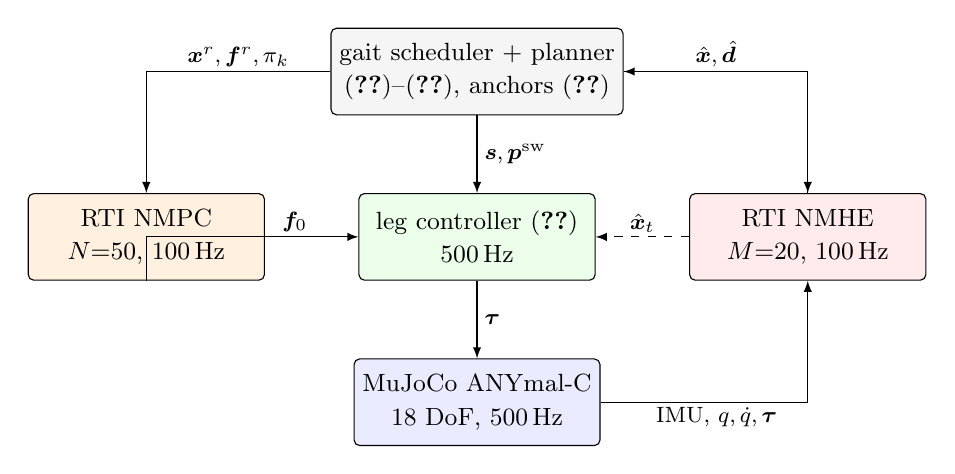
\begin{tikzpicture}[>=latex,font=\small,
  box/.style={draw,rounded corners=2pt,align=center,minimum width=30mm,minimum height=11mm,inner sep=3pt,font=\small},
  lab/.style={font=\footnotesize,inner sep=1.5pt,fill=white}]
% --- nodes on a clean grid ---
\node[box,fill=gray!8]   (plan) at (0,4.2)   {gait scheduler + planner\\[1pt]\eqref{eq:gait}--\eqref{eq:swing}, anchors \eqref{eq:anchor}};
\node[box,fill=orange!12](mpc)  at (-4.2,2.1){RTI NMPC\\[1pt]$N{=}50$, 100\,Hz};
\node[box,fill=red!8]    (mhe)  at ( 4.2,2.1){RTI NMHE\\[1pt]$M{=}20$, 100\,Hz};
\node[box,fill=green!8]  (ll)   at (0,2.1)   {leg controller \eqref{eq:torque}\\[1pt]500\,Hz};
\node[box,fill=blue!8]   (plant)at (0,0)     {MuJoCo ANYmal-C\\[1pt]18 DoF, 500\,Hz};
% --- planner outputs ---
\draw[->] (plan.west) -| (mpc.north) node[lab,pos=0.25,above]{$\bx^r,\bfv^r,\pi_k$};
\draw[->] (plan.east) -| (mhe.north);
\draw[->] (plan.south) -- (ll.north) node[lab,midway,right=1pt]{$\bs,\bp^{\mathrm{sw}}$};
% --- control path ---
\draw[->] (mpc.south) |- (ll.west) node[lab,pos=0.85,above]{$\bfv_0$};
\draw[->] (ll.south) -- (plant.north) node[lab,midway,right=1pt]{$\bm\tau$};
% --- estimation path ---
\draw[->] (plant.east) -| (mhe.south) node[lab,pos=0.28,below]{IMU, $q,\dot q,\bm\tau$};
\draw[->] (mhe.north) |- (plan.east) node[lab,pos=0.75,above]{$\hat\bx,\hat\bd$};
% --- fast estimate straight to the leg controller ---
\draw[->,dashed] (mhe.west) -- (ll.east) node[lab,midway,above]{$\hat\bx_t$};
\end{tikzpicture}
\caption{Unified loop. The planner is the only component that sees both solvers; it turns the NMHE state into the NMPC references, stage parameters and swing targets, and anchors feet from the estimate. The dashed arrow indicates that the estimate reaches the NMPC through the planner.}
\label{fig:arch}
\end{figure}

\begin{table}[t]\centering\caption{Rates and dimensions of the loop.}\label{tab:rates}
\footnotesize\begin{tabular}{@{}lccl@{}}\toprule
Component & rate & dims & notes\\\midrule
MuJoCo plant & 500 Hz & $n_q=19,n_v=18$ & torque actuators, $\pm80$ Nm\\
leg controller & 500 Hz & 12 & \eqref{eq:torque}\\
RTI NMHE & 100 Hz & $18/6/21/33/28/16$ & $n_x/n_w/n_y/n_u/n_c/n^M_c$, $M=20$\\
RTI NMPC & 100 Hz & $12/12/28/0$ & $n_x/n_u/n_c/n^N_c$, $N=50$\\
planner & 100 Hz & --- & shares $\hat\bx$ with both\\
\bottomrule\end{tabular}\end{table}

\subsubsection{Ordering within a sample}
At a 10~ms boundary the driver (i) forms the measurement \eqref{eq:h}, detects contacts, updates the anchors and gates and runs the estimator cycle, (ii) builds references and stage parameters from the fresh estimate and runs the controller cycle, (iii) starts accumulating the realised GRF for the next interval input. The interval input must be the force applied \emph{after} the NMPC update of the same instant; using the pre-update force (a one-sample staleness) produced spurious 40~Nm torque disturbances at every force change and was the first bug found in closed loop.

\subsubsection{Latency budget}
Both solvers expose an instantaneous output: the controller's first input is available 0.11~$\mu$s after the estimate, and the estimator's innovation-based estimate $\hat\bx^{\mathrm{fast}}_t$ 1.1~$\mu$s after the measurement. The measurement-to-actuation latency of the joint loop is therefore dominated by the leg controller's 2~ms period and the NMHE's smoothing feedback (37~$\mu$s), not by the optimisation: the sample ordering of Algorithm~\ref{alg:loop} places the two instantaneous outputs back to back so that a fresh GRF command reaches the joints $\approx0.3$~ms after the sensors were read, with the remaining $\approx0.5$~ms of NMPC preparation for the \emph{next} sample overlapping the plant's motion---the RTI prepare/feedback split at the system level. Figure~\ref{fig:timeline} illustrates the schedule.

\begin{figure}[t]\centering
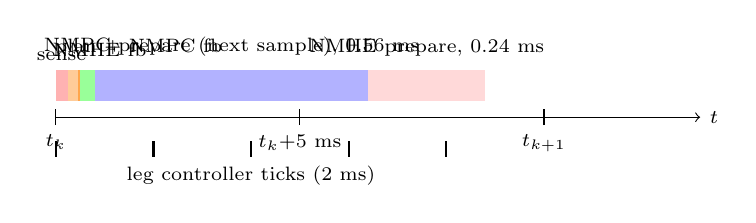
\begin{tikzpicture}[font=\scriptsize,x=0.62cm]
\draw[->] (0,0) -- (13.2,0) node[right]{$t$};
\foreach \x in {0,5,10} {\draw (\x,-0.1)--(\x,0.1);}
\node[below] at (0,-0.1){$t_k$}; \node[below] at (5,-0.1){$t_k{+}5$ ms}; \node[below] at (10,-0.1){$t_{k+1}$};
\fill[red!30] (0,0.2) rectangle (0.25,0.6); \node[above] at (0.12,0.6){sense};
\fill[orange!40] (0.25,0.2) rectangle (0.45,0.6); \node[above,rotate=0] at (0.9,0.65){NMHE fb};
\fill[orange!70] (0.45,0.2) rectangle (0.5,0.6);
\fill[green!40] (0.5,0.2) rectangle (0.8,0.6); \node[above] at (1.7,0.65){plan + NMPC fb};
\fill[blue!30] (0.8,0.2) rectangle (6.4,0.6); \node[above] at (3.6,0.65){NMPC prepare (next sample), 0.56 ms};
\fill[red!15] (6.4,0.2) rectangle (8.8,0.6); \node[above] at (7.6,0.65){NMHE prepare, 0.24 ms};
\foreach \x in {0,2,4,6,8} {\draw[thick] (\x,-0.5)--(\x,-0.3);} \node[below] at (4,-0.5){leg controller ticks (2 ms)};
\end{tikzpicture}
\caption{Schedule of one 10~ms sample (not to scale within the first millisecond). Sensing, the estimator feedback, planning and the controller feedback complete in $\approx0.3$~ms; both preparations for the next sample overlap the plant's motion.}
\label{fig:timeline}
\end{figure}

\subsubsection{Disturbance feed-forward}
The NMPC receives $\bd=(\hat\bd_f,\bm0)$ for all stages: the estimated force is fed forward, the estimated torque is not. The torque channel is estimated with a within-trot standard deviation of 4--6~Nm (the reaction of the swinging legs on the trunk, which the SRBD does not model) and its feed-forward closed a positive-feedback loop through the roll dynamics that doubled the roll excursion and quadrupled the NMPC's inner-iteration load (Table~\ref{tab:ablation}); the force channel is smooth (2--3~N within trot) and its feed-forward reduces the drift under the lateral push by a factor of five. This is a bandwidth statement, not a solver limitation: a disturbance observer should only be closed over frequencies it estimates faithfully.

\section{Verification}
\subsection{Model and derivatives}
The generated C model was checked at random points against (i) the SymPy expressions it was generated from ($1.7\times10^{-13}$ maximum deviation, $8.5\times10^{-14}$ for the augmented set), (ii) central finite differences of all Jacobians, including the RK4 chain rule for the discrete $A_k,B_k$ ($2.5$--$3.2\times10^{-9}$ relative), and (iii) each other: the controller's dynamics $f_c(\bx,\bfv;\pi)$ and the first twelve rows of the estimator's augmented dynamics agree bitwise for the same arguments, which is the operational meaning of ``one model source''.

\subsection{Model consistency on the plant}
The SRBD residual $m\,\Delta\bv/h-\sum_i\bfv^{\mathrm{meas}}_i-m\bm g$ evaluated with the interval-mean realised forces of the closed-loop run is zero-mean ($<0.05$~N in all axes over 6~s of trot) with standard deviation $(22,6,29)$~N and isolated single-sample spikes of up to $(132,36,169)$~N at touchdowns---the velocity jump of the landing leg's mass, which the lumped model attributes to the trunk. The torque balance with the commanded forces and the true attitude closes to 0.6~Nm rms while standing. These numbers bound what the disturbance state has to absorb and confirm the sign and frame conventions of \eqref{eq:srbd}.

\subsection{Fixed-parameter convergence of the NMPC}
At a mid-swing instant of the walk ($t=2.35$~s, LF/RH in stance, two contact switches inside the horizon) the iteration was run at frozen $\hat\bx$ from a cold start ($\bfv\equiv0$) and from the weight-distributing warm start of \eqref{eq:uref}. The KKT residual decreases as $1.1\times10^{1}\to1.4\times10^{-1}\to2.0\times10^{-3}\to1.4\times10^{-5}\to7.4\times10^{-8}\to4.1\times10^{-10}$ (cold) and $6.0\times10^{-2}\to1.2\times10^{-2}\to2.2\times10^{-5}\to7.3\times10^{-7}\to1.5\times10^{-9}\to4.0\times10^{-11}$ (warm), \ie\ six cycles to $10^{-10}$ in both cases with a contraction factor of $\approx10^{-2}$ per cycle (Fig.~\ref{fig:conv}). The cold and warm starts converge to the same solution, including the same set of constraints active at the contact switches inside the horizon, which is the check that the warm start used in closed loop is not biasing the solution. In closed loop the one-cycle KKT residual stays at $7$--$8\times10^{-2}$ in the unnormalised units of \eqref{eq:ocp} ($\approx10^{-3}$ relative to the cold-start value) and the maximum constraint violation of the committed input is $3.8\times10^{-2}$ in normalised units (8.6~N on a 400~N cone edge, one sample, at a touchdown).

\subsection{Estimator mode consistency}
The estimator can re-linearise every stage of the window at every sample, or re-use stage information that the window structure makes re-usable. Running both modes on an identical plant trajectory (ground-truth-fed control, so that both see the same data) gives estimates whose rms errors agree to four significant digits in every component, with a maximum pointwise difference of $1.3\times10^{-4}$ (state, SI units) and $9.6\times10^{-3}$~N (wrench) over 800 samples, while the preparation phase costs $215$~$\mu$s instead of $1170$~$\mu$s. The cheaper mode is used in all closed-loop runs; the agreement is the check that it is not trading accuracy for speed.
\section{Closed-Loop Results}
\subsection{Setup}
Plant: MuJoCo 3.13, ANYmal-C from the Menagerie with the position servos replaced by direct torque motors ($\pm80$~Nm) and the foot contacts stiffened (\texttt{solimp 0.9 0.95 0.001}, \texttt{solref 0.005 1}, $\mu_{\mathrm{plant}}=0.8$; the Menagerie's soft feet, \texttt{solimp 0.015 1 0.03}, creep laterally under sustained load and bias leg odometry by 25\,\%), 2~ms time step, joint damping 1~Nms/rad and dry friction 0.1~Nm as shipped. Sensor noise (white, per sample): attitude 5~mrad, gyro 0.02~rad/s, joint velocities 0.05~rad/s, forward kinematics 3~mm, realised GRF 2~N. Scenario: stand for 1~s; ramp a forward command to 0.4~m/s over 1~s and trot; lateral push of 40~N on the trunk for 0.8~s from $t=3.5$~s; yaw-rate command 0.3~rad/s from $t=5$~s; end at 8~s. Timing host: shared cloud vCPU (Intel Xeon, 2.8~GHz class), gcc 13 \texttt{-O3 -march=native}, single core, wall-clock per call via \texttt{clock\_gettime}; the simulator, renderer and Python driver share the core, so the numbers are conservative relative to an isolated single-core measurement.

\subsection{Main run}
Figure~\ref{fig:tracking} shows the closed-loop tracking, Fig.~\ref{fig:esterr} the estimation errors, Fig.~\ref{fig:dist} the estimated wrench, and Fig.~\ref{fig:sheet} frames of the animation. In steady trot the forward speed is $0.32\pm0.02$~m/s during the ramp-out phase (2.5--3.5~s) and $0.38$~m/s in the turn, against a 0.4~m/s command; the deficit is consistent with the $-5$~N per foot longitudinal drag of the plant's joint damping and friction, which appears in the estimated $\hat d_{f,x}$ as $+1.9$~N (net of the feed-forward). Roll stays within $\pm0.09$~rad and pitch within $\pm0.06$~rad over the whole run including push and turn; height is $0.452\pm0.002$~m against $0.45$~m commanded. The yaw rate settles at $0.28$~rad/s for a 0.3~rad/s command; during the turn the body-frame lateral velocity drifts to $-0.2$ to $-0.4$~m/s, \ie\ the heading is tracked but the velocity vector lags it and the robot crabs partly sideways along the arc---a limitation of the foothold heuristic \eqref{eq:raibert}, which places feet from the current velocity rather than from the commanded arc, not of the solvers. Estimation errors (rms over $t>1.5$~s): position $(1.0,0.5,0.4)$~cm (odometry drift, not noise), attitude $(1.4,2.6,1.7)$~mrad, velocity $(9,10,7)$~mm/s, angular velocity $(0.19,0.07,0.07)$~rad/s---the roll-rate error being the trot's 10--20~Hz roll vibration which the SRBD does not predict and the gyro row (0.05~rad/s) smooths. The 40~N push is estimated at $39.5$~N (mean over its last 0.5~s) with the $0.3$~s rise time expected from $W$, and the estimate returns to $-1.4$~N within 0.3~s after release. Within-trot wrench fluctuations are $(2.9,2.2,2.1)$~N and $(5.8,3.7,5.4)$~Nm.

\begin{figure*}[t]\centering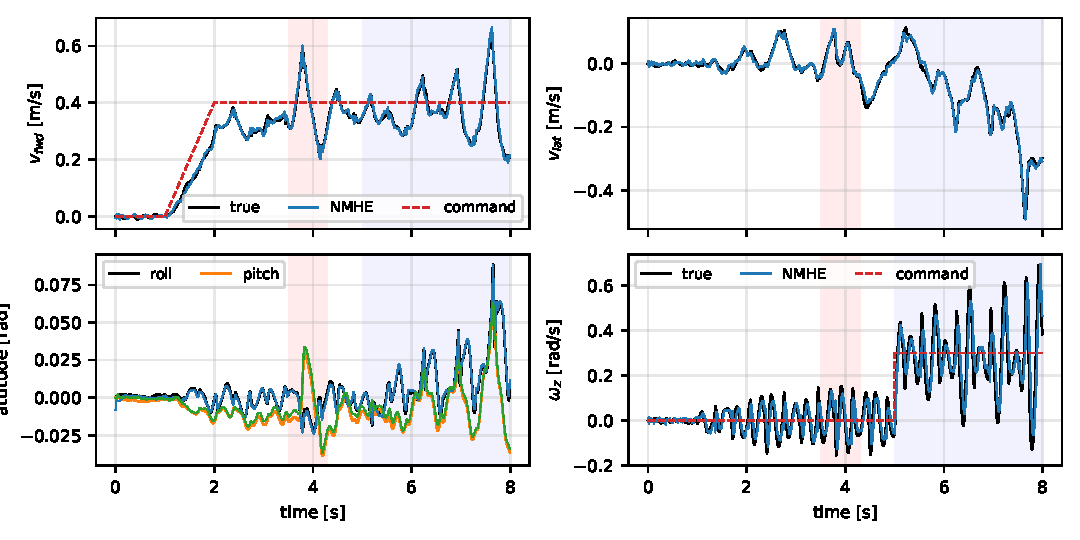
\includegraphics[width=\textwidth]{tracking.pdf}
\caption{Main run: body-frame forward and lateral velocity, attitude and yaw rate; true (black), NMHE estimate (blue/green), commands (dashed). Shaded: push (red), turn (blue).}\label{fig:tracking}\end{figure*}
\begin{figure*}[t]\centering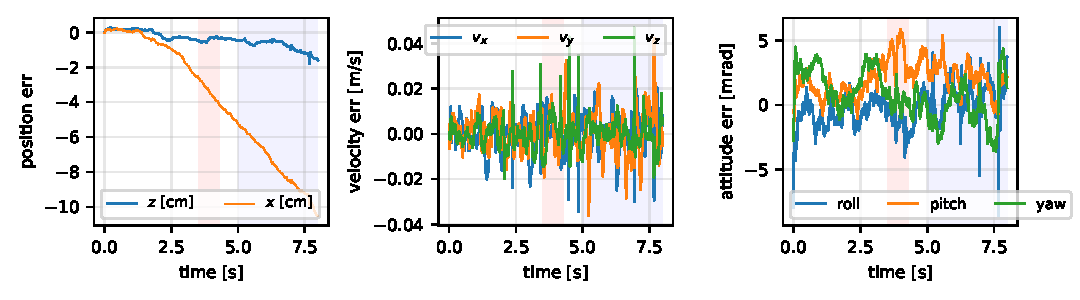
\includegraphics[width=\textwidth]{est_err.pdf}
\caption{Main run: estimation errors of the smoothed NMHE output. Position drifts (leg odometry is dead reckoning); velocity and attitude do not.}\label{fig:esterr}\end{figure*}
\begin{figure*}[t]\centering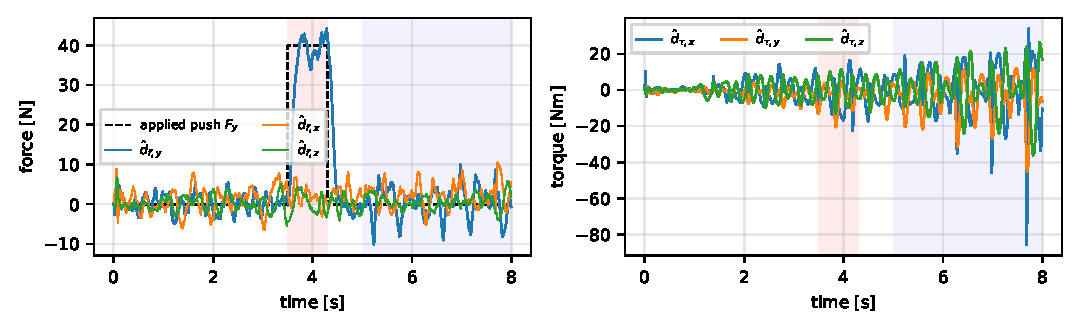
\includegraphics[width=\textwidth]{disturbance.pdf}
\caption{Main run: estimated wrench state $\hat\bd$. The 40~N lateral push (dashed) is recovered by the augmented random-walk state; the torque channel carries the swing-leg reaction at the gait frequency.}\label{fig:dist}\end{figure*}
\begin{figure*}[t]\centering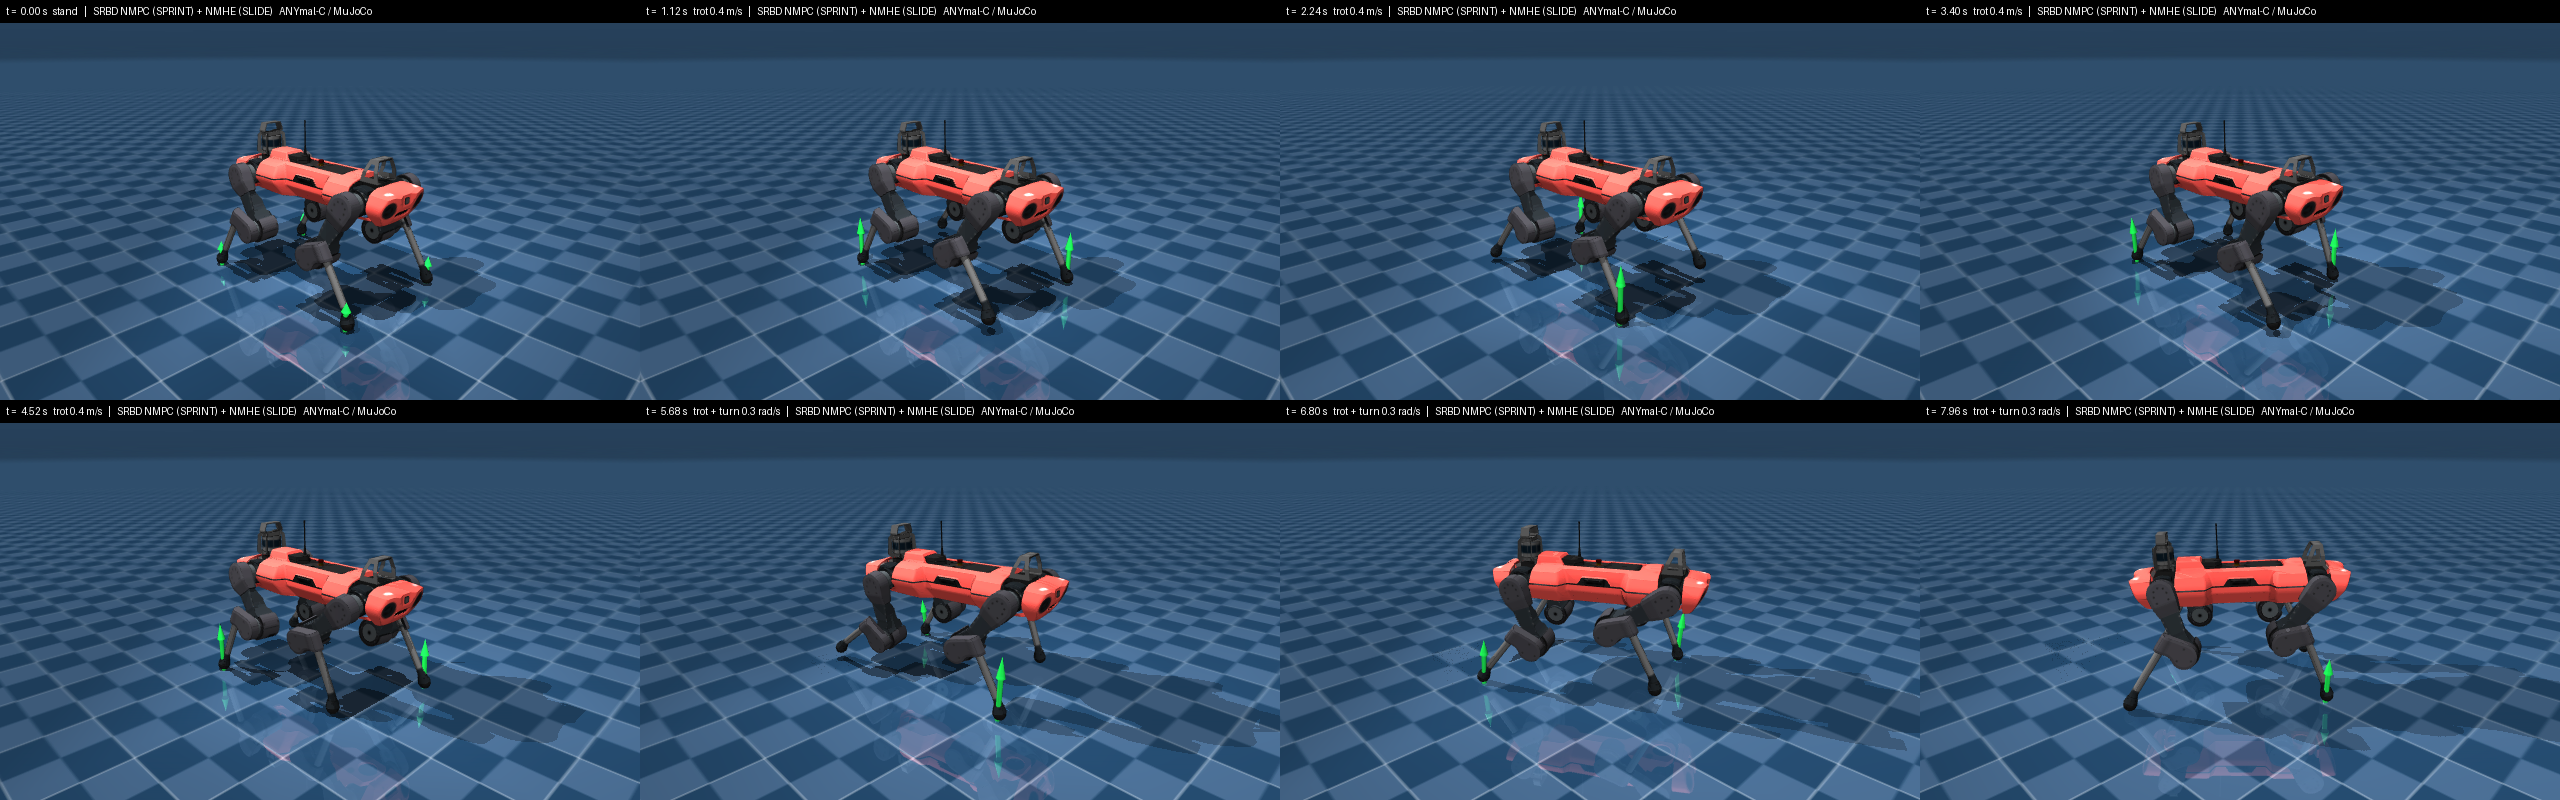
\includegraphics[width=\textwidth]{contact_sheet.png}
\caption{Frames from the released animation (\texttt{media/anymal\_walk\_hd.mp4}): stand, trot, push, turn. Green arrows are the commanded ground reaction forces $\bfv_i$ (scaled 1~m~$\equiv$~400~N), the red arrow the push.}\label{fig:sheet}\end{figure*}

\subsection{Force commands and the predicted horizon}
Figure~\ref{fig:grf} compares commanded and realised GRFs over one gait cycle: the diagonal pair carries $\approx210$--$230$~N per foot vertically with $|f_x|\le20$~N, the commands stay inside the pyramid with margin, and the realised forces follow to within the touchdown transient (the first 20--40~ms of each stance) and the leg-inertia term of Sec.~III-E. Figure~\ref{fig:horizon} shows one NMPC solution: the horizon spans two contact switches, the predicted height rises 1~mm over 0.5~s towards its reference (the NMPC's height loop is proportional; offset removal is left to the disturbance feed-forward), and the force plan hands the load over between the diagonal pairs at the switches without transient---the warm start \eqref{eq:uref} and the shifted iterate make a contact switch a non-event for the solver, which is why the inner loop runs a second pass on only 3\,\% of the samples.

\begin{figure}[t]\centering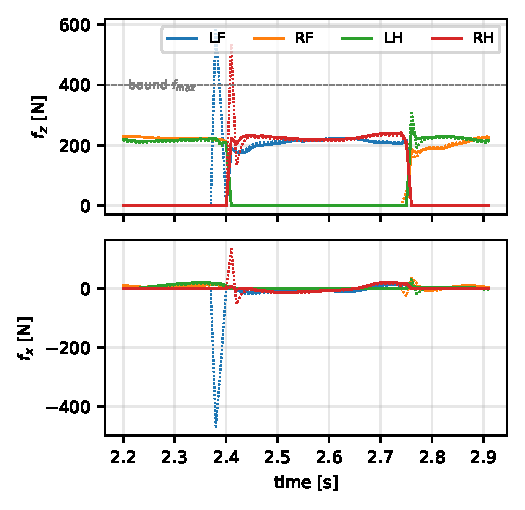
\includegraphics[width=0.86\textwidth]{grf.pdf}
\caption{Commanded (solid) and realised (dotted) vertical and longitudinal GRFs over one gait cycle of the main run.}\label{fig:grf}\end{figure}
\begin{figure}[t]\centering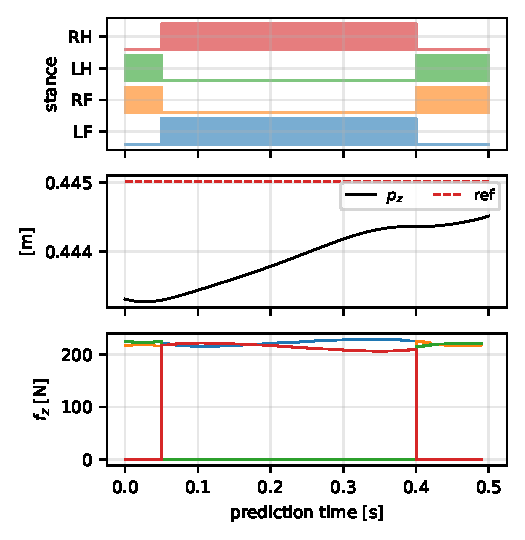
\includegraphics[width=0.86\textwidth]{horizon.pdf}
\caption{One NMPC solution ($t=2.35$~s): predicted contact schedule, height, and vertical force plan over the 0.5~s horizon.}\label{fig:horizon}\end{figure}

\subsection{Timing}
Table~\ref{tab:timing} and Fig.~\ref{fig:timing} give the per-sample distributions. The NMPC preparation ($0.56$~ms median, $0.71$~ms p99, $1.07$~ms max) is dominated by the linearisation of 50 stages; its feedback ($56$~$\mu$s median) includes an occasional second inner pass (p99 $194$~$\mu$s, max $412$~$\mu$s at contact switches). The applied-input latency is $0.11$~$\mu$s. The NMHE preparation ($0.24$~ms median) covers the linearisation of the window; its instantaneous output costs $1.1$~$\mu$s and the smoothed feedback $37$~$\mu$s. One complete estimate-then-control cycle therefore costs $\approx0.9$~ms median and $\le2.1$~ms worst case against the 10~ms period, on a shared core, in plain C without SIMD---roughly 9\,\% utilisation with a $5\times$ worst-case margin.

\subsubsection{Horizon scaling}
Rebuilding the NMPC for $N\in\{10,20,30,50,80,120\}$ (same $h$, same weights) and timing it on the walking scenario gives Table~\ref{tab:scaling}: preparation and feedback are affine in $N$ with slopes of $10.9$ and $1.15$~$\mu$s per stage and the applied-input latency is flat at $0.1$~$\mu$s, as expected for a stage-wise structured solver; memory grows by $16.0$~kB per stage. All horizons from 0.1~s upward trot stably at 0.3~m/s on this scenario (no push); $N=120$ (1.2~s) walks slower because a reference arc re-anchored at the current position is a poor description of the gait that far ahead. The choice $N=50$ is a comfortable 0.7 gait cycles at 5\,\% of the period.

\begin{table}[t]\centering\caption{NMPC horizon scaling on the walking scenario (medians over 300 samples; times in $\mu$s, memory in kB).}\label{tab:scaling}
\footnotesize\begin{tabular}{@{}rrrrrrr@{}}\toprule
$N$ & horizon [s] & prep & prep p99 & feedback & $u_0$ latency & RAM\\\midrule
10 & 0.1 & 113 & 156 & 11.7 & 0.11 & 168\\
20 & 0.2 & 220 & 263 & 22.1 & 0.12 & 328\\
30 & 0.3 & 311 & 359 & 31.7 & 0.10 & 488\\
50 & 0.5 & 531 & 656 & 54.5 & 0.11 & 809\\
80 & 0.8 & 889 & 1184 & 90.4 & 0.12 & 1290\\
120 & 1.2 & 1304 & 1759 & 136.8 & 0.12 & 1931\\
\bottomrule\end{tabular}\end{table}

\begin{table}[t]\centering\caption{Per-sample wall times [$\mu$s] in the main run (800 NMPC and 800 NMHE cycles) and static memory.}\label{tab:timing}
\scriptsize\begin{tabular}{@{}llrrrl@{}}\toprule
solver & phase & med & p99 & max & \\\midrule
\multirow{3}{*}{NMPC} & preparation & 564 & 708 & 1065 & 809 kB\\
 & feedback & 56 & 194 & 412 & \\
 & $u_0$ latency & 0.11 & & & \\\midrule
\multirow{4}{*}{NMHE} & preparation & 241 & 560 & 1019 & 579 kB\\
 & prep.\ (full relin.) & 1190 & 1468 & 1840 & \\
 & instant output & 1.1 & & & \\
 & feedback & 37 & 68 & 423 & \\
\bottomrule\end{tabular}\end{table}
\begin{figure}[t]\centering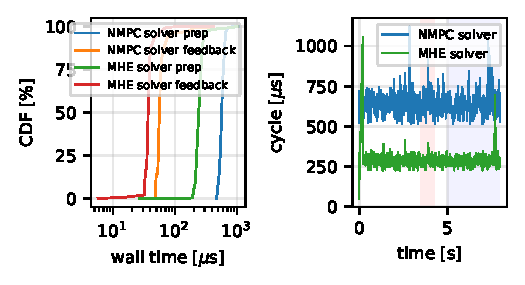
\includegraphics[width=0.86\textwidth]{timing.pdf}
\caption{Left: empirical CDFs of the per-sample phases. Right: complete cycle times along the run; the NMPC's bursts are contact-switch samples with a second inner pass.}\label{fig:timing}\end{figure}
\begin{figure}[t]\centering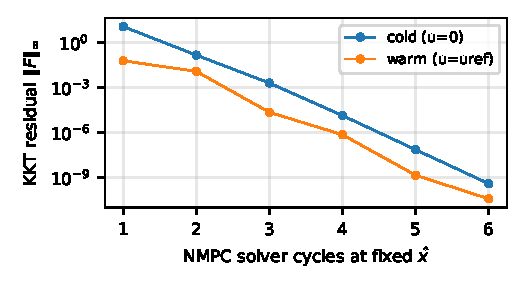
\includegraphics[width=0.86\textwidth]{convergence.pdf}
\caption{Fixed-parameter convergence on the walking OCP at $t=2.35$~s from a cold and a warm start.}\label{fig:conv}\end{figure}

\subsection{Ablations}
Table~\ref{tab:ablation} and Fig.~\ref{fig:ablation} compare, on the same seed and scenario: (a) ground-truth state feedback (no estimator), (b) the NMHE without feed-forward, (c) force feed-forward (the proposed configuration), (d) full wrench feed-forward, and (e) the NMHE in exact mode. Two observations. First, the estimator costs essentially nothing in nominal control performance: roll and pitch excursions with the NMHE (0.09/0.06~rad) are within a factor two of the truth-fed run (0.04/0.05~rad) and the forward speed is higher (0.32 vs 0.29~m/s), because the estimated drag is fed forward. Second, feed-forward of the estimated force is what turns the push from a 0.74~m lateral excursion (uncompensated, 0.26~m with truth feedback) into 0.15~m, while feed-forward of the torque as well degrades everything (roll 0.18~rad, speed overshoot to 0.64~m/s in the turn, NMPC feedback p99 of 1.1~ms from inner-iteration churn). The exact-mode NMHE reproduces the reuse-mode run to the resolution of the table at five times the estimator cost.

\begin{table*}[t]\centering\caption{Ablations on the main scenario (seed 0). Extremes over $t>1.5$~s; $p_y$ at the end of the push ($t=4.3$~s) and at $t=8$~s; estimation rms over $t>1.5$~s; NMPC feedback p99 [$\mu$s].}\label{tab:ablation}
\scriptsize\resizebox{\textwidth}{!}{\begin{tabular}{@{}lcccccccccc@{}}\toprule
configuration & roll max & pitch max & $z_{\min}$ & $z_{\max}$ & $v_{fwd}$ walk/turn & $\dot\psi$ turn & $p_y$ push/end & $\hat\bv$ rms [mm/s] & $\hat\bth$ rms [mrad] & fb p99\\\midrule
truth-fed control (no NMHE) & 0.044 & 0.047 & 0.445 & 0.457 & 0.29/0.29 & 0.29 & 0.26/0.70 & --- & --- & 189\\
NMHE, no feed-forward & 0.073 & 0.051 & 0.448 & 0.462 & 0.32/0.41 & 0.28 & 0.24/0.74 & (9,10,8) & (1.5,2.6,1.7) & 180\\
NMHE, force feed-forward (proposed) & 0.089 & 0.063 & 0.448 & 0.464 & 0.32/0.38 & 0.28 & 0.03/0.15 & (9,10,7) & (1.4,2.6,1.7) & 194\\
NMHE, full wrench feed-forward & 0.176 & 0.211 & 0.444 & 0.503 & 0.38/0.64 & 0.19 & 0.05/0.33 & (22,32,18) & (1.7,2.5,1.7) & 1110\\
NMHE exact mode, force feed-forward & 0.094 & 0.066 & 0.448 & 0.464 & 0.32/0.38 & 0.28 & 0.03/0.15 & (9,10,7) & (1.4,2.6,1.7) & 216\\
\bottomrule\end{tabular}}\end{table*}
\begin{figure}[t]\centering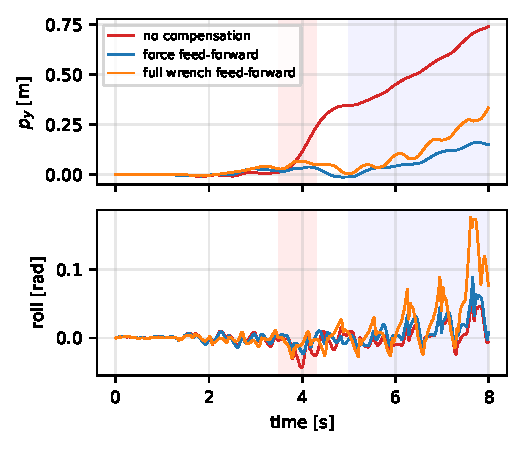
\includegraphics[width=0.86\textwidth]{ablation.pdf}
\caption{Push recovery: lateral position and roll for no / force / full wrench feed-forward.}\label{fig:ablation}\end{figure}

\subsection{Sensitivity to sensor noise}
Scaling all sensor noises jointly by a factor $\alpha\in\{0,\tfrac12,1,2,4\}$ (nominal: attitude 5~mrad, gyro 0.02~rad/s, joint velocities 0.05~rad/s, forward kinematics 3~mm, GRF 2~N) gives Table~\ref{tab:noise}. Estimation errors grow essentially linearly with $\alpha$ up to $\alpha=2$ (velocity 4~mm/s noise-free to 16~mm/s at $\alpha=2$; attitude 0.8 to 2.6~mrad), the push estimate stays within 4\,\% of 40~N, and the closed loop remains stable with roll excursions growing from 0.06 to 0.13~rad. At $\alpha=4$ (20~mrad attitude, 0.08~rad/s gyro, 0.2~rad/s joint velocities, 12~mm kinematics, 8~N forces) the loop falls during the turn: the roll-rate estimate error reaches 1~rad/s and the NMPC, which sees the noisy roll rate through $Q_\omega$, over-reacts. The noise-free run is not better than the nominal one in control performance (roll 0.06 vs 0.09~rad), confirming that the nominal sensor noise is not what limits the loop; the SRBD residual is.

\begin{table}[t]\centering\caption{Joint sensor-noise scaling $\alpha$, proposed configuration, seed 0. Errors are rms over $t>1.5$~s; push estimate is the mean $\hat d_{f,y}$ over the last 0.5~s of the 40~N push.}\label{tab:noise}
\scriptsize\setlength\tabcolsep{3pt}\begin{tabular}{@{}cccccccc@{}}\toprule
$\alpha$ & fall & roll & $\hat\bv$ [mm/s] & $\hat\bth$ [mrad] & $\hat\omega_x$ & $\hat z$ [mm] & push [N]\\\midrule
0 & no & 0.059 & (4,7,4) & (0.8,1.4,1.3) & 0.16 & 1.1 & 40.7\\
0.5 & no & 0.071 & (5,7,5) & (1.0,2.1,1.2) & 0.17 & 3.7 & 40.0\\
1 & no & 0.089 & (9,10,7) & (1.4,2.6,1.7) & 0.19 & 6.4 & 39.5\\
2 & no & 0.126 & (16,17,13) & (2.6,4.0,3.4) & 0.24 & 9.7 & 38.5\\
4 & yes ($t\approx7$ s) & --- & --- & --- & 1.07 & --- & 35.7\\
\bottomrule\end{tabular}\end{table}

\subsection{Robustness over noise seeds and what it took}
Five independent noise realisations complete the full scenario without a fall: roll maxima $0.03$--$0.09$~rad, pitch $0.05$--$0.06$~rad, forward speed $0.28$--$0.32$~m/s during the ramp-out, yaw rate $0.27$--$0.29$~rad/s, push excursion $0.03$--$0.13$~m, velocity rms $\le12$~mm/s (Table~\ref{tab:seeds}). Table~\ref{tab:lessons} lists, in the order they were found, the modelling decisions that separated a loop that falls within two strides from one that walks; each was isolated by comparing ground-truth-fed and estimator-fed closed loops and estimator-only runs on identical trajectories. None of them required a change to either kernel; all of them are recorded because a reader porting the framework to another robot will meet them again.

\begin{table}[t]\centering\caption{Five noise seeds, proposed configuration.}\label{tab:seeds}
\scriptsize\begin{tabular}{@{}lccccccc@{}}\toprule
seed & fall & roll max & pitch max & $v_{fwd}$ & $\dot\psi$ & $p_y$ push & $\hat\bv$ rms [mm/s]\\\midrule
0 & no & 0.089 & 0.063 & 0.32 & 0.28 & 0.03 & (9,10,7)\\
1 & no & 0.031 & 0.048 & 0.28 & 0.29 & 0.13 & (8,11,6)\\
2 & no & 0.038 & 0.047 & 0.30 & 0.28 & 0.12 & (10,12,7)\\
3 & no & 0.080 & 0.054 & 0.31 & 0.27 & 0.04 & (10,11,7)\\
4 & no & 0.071 & 0.055 & 0.30 & 0.29 & 0.06 & (10,10,6)\\
\bottomrule\end{tabular}\end{table}

\begin{table*}[t]\centering\caption{Development ablations (chronological): symptom, cause, fix, and effect. ``Truth-fed'' = NMPC on ground-truth state; ``est-only'' = estimator run on a truth-fed closed loop.}\label{tab:lessons}
\footnotesize\begin{tabular}{@{}p{3.2cm}p{4.7cm}p{4.2cm}p{3.0cm}@{}}\toprule
Symptom & Cause & Fix & Effect\\\midrule
Standing loop rolls at 25~Hz with NMHE, stable truth-fed & NMHE interval input was the force \emph{before} the NMPC update of the same instant (one-sample stale) & accumulate realised force after the update & spurious $\pm40$~Nm torque estimate removed\\
Body rises 5--9~cm in trot & $\tau=-J\T\bfv$ ignores leg gravity: realised GRF $=\bfv+J^{-\mathsf T}\bm b$ & add bias torques in stance \eqref{eq:torque} & realised$-$commanded $-1$~N mean\\
540--590~N impacts at touchdown & $\sin(\pi\sigma)$ swing height has $-0.5$~m/s end slope; targets in sphere-centre frame vs contact-point feedback (3~cm late) & bump profile, $z_{\mathrm{land}}=-1.5$~cm, consistent frame & impacts $\le170$~N single-sample\\
Speed 0.17--0.25 for 0.4 m/s command; $T_g=0.5$--$0.6$~s unstable & foot placed ahead of the sweep (neutral point from commanded velocity) & neutral point from actual velocity, $T_g=0.7$~s, $k_r$ 0.05--0.12 & 0.32--0.38 m/s\\
$\hat z$ jumps $+1$~cm per touchdown, $\hat v$ spikes 2~m/s & kinematic velocity from a foot still moving; anchors from a foot still sliding & settled-stance gates \eqref{eq:gate}, contact detection, contact-point Jacobians & $\hat z$ max error 1.7~cm\\
$\hat z$ drifts $-2.5$~cm per stride in closed loop only & scheduled-stance force gating dropped early-contact forces (1.5 cm overshoot lands early) & $s^{\mathrm{dyn}}=\max(s,\delta)$, anchor at detection & drift 2~cm over 5~s\\
Push estimated at 36--40 of 60~N; velocity lags 40\,\% & disturbance modelled as a penalised estimator input is weakly observable over one interval (Sec.~V-A) & random-walk wrench state \eqref{eq:aug} & 61.8~N, no lag\\
$-2.3$~cm/s forward-velocity bias & anchoring from the filtered estimate inherits estimator lag; $\sigma_v=0.1$ too weak & $\sigma_v=0.03$, $\sigma_\rho=0.01$ & bias $<1$~mm/s\\
Falls after push with full wrench feed-forward & torque channel carries gait-frequency swing reaction; feed-forward closes a roll loop & feed forward force only & roll 0.09 vs 0.18~rad\\
Speed runaway to 0.9~m/s while turning & world-frame velocity command integrated while the body yaws & body-frame command along the arc \eqref{eq:refs} & 0.38~m/s, $\dot\psi$ 0.28\\
\bottomrule\end{tabular}\end{table*}

\section{Discussion and Limitations}
\emph{What the SRBD costs on this robot.} With the legs carrying 57\,\% of the mass, the lumped model is coarse: the touchdown residuals of Sec.~VII-C, the gait-frequency torque channel of Fig.~\ref{fig:dist}, the $0.19$~rad/s roll-rate estimation error and the 5--10\,\% speed deficit are all leg-mass effects. They are absorbed by three mechanisms that this report makes explicit---realised forces as known inputs, the augmented wrench state, and the choice of what to feed forward---rather than hidden in tuning. A centroidal or kino-dynamic model would remove most of them at the price of a $n_x\ge24$ NMPC; nothing in the solver interfaces prevents that extension, and the stage-parameter mechanism carries over unchanged.

\emph{Contact softness.} Leg odometry assumes stationary feet; compliant contacts violate it. The Menagerie's soft feet gave a 25\,\% velocity bias that no estimator can correct without modelling the compliance; we stiffened the plant, which is the honest choice for a study of the estimator rather than of the contact model. Real ANYmal feet are stiff; real ground is not always.

\emph{Odometry drift and yaw.} Absolute position and, strictly, yaw are unobservable from proprioception; the AHRS row supplies yaw here. Position drifted 2~cm over 5~s in the main run---an artefact of the anchoring rule \eqref{eq:anchor}, not of the solver---and is irrelevant for velocity-commanded locomotion.

\emph{No external optimality oracle.} IPOPT was not available in the build environment. Optimality is therefore established by the fixed-parameter convergence of Sec.~VII-D (to $10^{-10}$ KKT residual from a cold start) and by the agreement of the two estimator linearisation modes in Sec.~VII-E, not by a third-party solve. The release contains the CasADi model builders that the companion papers use for their IPOPT oracles, so the check can be run where IPOPT is installed.

\emph{Constraint semantics.} The stage inequalities are enforced by the solver as penalised constraints and can be transiently violated during fast transients; the largest violation of a committed input was 8.6~N on a 400~N cone edge, for one sample, at a touchdown. Applications requiring strict inviolability should tighten $\mu$ or add a projection at the leg-controller level.

\emph{Timing.} The reported times include Python/MuJoCo contention on a shared cloud core and are conservative. The per-sample cost of the NMPC grows linearly in the horizon (Table~\ref{tab:scaling}) and that of the NMHE is constant in the window length, which is what makes the 10~ms budget comfortable. Both would benefit from blocked linear-algebra kernels and SIMD, and the NMPC from a shorter horizon at a coarser stage length (25 stages of 20~ms cover the same 0.5~s at half the cost; the 20~ms period was abandoned here only because the first tuning was too aggressive for it).

\emph{Towards the real robot.} The framework's interface to a physical ANYmal is small: joint angles, velocities and torques at 500~Hz, an AHRS attitude and gyro, and a contact-detection threshold. The realised-GRF reconstruction $-J_i^{-\mathsf T}(\bm\tau^{\mathrm{meas}}_i-\bm b_i)$ uses the same leg model as the controller and is standard on torque-controlled quadrupeds; the AHRS yaw can be replaced by integrating the gyro if no magnetometer is available (yaw then drifts like position, which the velocity-commanded loop tolerates). The two kernels' static memory (809~kB and 579~kB) and worst-case cycle times ($\le2.1$~ms together on a shared core) fit any onboard computer; on a Cortex-A class embedded target the $N$-scaling of Table~\ref{tab:scaling} suggests $N=30$ (0.3~s) as a safe choice, which walked as well as $N=50$ in the horizon sweep.

\section{Conclusion}
A single symbolic SRBD model, instantiated once as an RTI NMPC with gait-scheduled stage parameters and once as an RTI moving-horizon estimator with an augmented wrench state and a known-input encoding of the contact situation, closes an output-feedback trot on a full-body ANYmal-C simulation with millisecond-scale solver cycles, centimetre-per-second velocity estimates, and a disturbance observer accurate enough to feed forward. Both solver libraries were used unmodified, behind an interface small enough that another RTI package can be substituted without touching the framework. One iteration per sample sufficed throughout: a second inner pass was needed on 3\,\% of the samples, all at contact switches. The engineering that made the loop work---realised forces as known inputs, settled-stance gating, anchoring at detection, bias-compensated torque mapping, force-only feed-forward---is documented as ablations so that it can be reused rather than rediscovered.

\appendix
\section{Jacobian structure of the SRBD model}
Writing $\bm m_i=\br_i-\bp$ and $\bm\tau=\sum_is_i\sk{\bm m_i}\bfv_i$ (world frame), the nonzero blocks of $\partial f_c/\partial\bx$ are
\begin{align*}
\frac{\partial\dot\bp}{\partial\bv}&=I,\qquad
\frac{\partial\dot\bth}{\partial\bom}=\Tm(\bth),\qquad
\frac{\partial\dot\bth}{\partial(\phi,\theta)}=\Big[\frac{\partial\Tm}{\partial\phi}\bom\ \ \frac{\partial\Tm}{\partial\theta}\bom\Big],\\
\frac{\partial\dot\bom}{\partial\bp}&=\I^{-1}\Rot\T\sum_i s_i\sk{\bfv_i},\qquad
\frac{\partial\dot\bom}{\partial\bth}=\I^{-1}\Big[\frac{\partial\Rot\T}{\partial\phi}\bm\tau\ \ \frac{\partial\Rot\T}{\partial\theta}\bm\tau\ \ \frac{\partial\Rot\T}{\partial\psi}\bm\tau\Big],\\
\frac{\partial\dot\bom}{\partial\bom}&=\I^{-1}\big(\sk{\I\bom}-\sk{\bom}\I\big),
\end{align*}
and of $\partial f_c/\partial\bfv$
\[
\frac{\partial\dot\bv}{\partial\bfv_i}=\frac{s_i}{m}I,\qquad \frac{\partial\dot\bom}{\partial\bfv_i}=s_i\,\I^{-1}\Rot\T\sk{\bm m_i},
\]
which vanish for swing feet. The augmented estimator model adds $\partial\dot\bv/\partial\bd_f=I/m$, $\partial\dot\bom/\partial\bd_\tau=\I^{-1}$ and $\partial\dot\bd/\partial\bw=I$. The output Jacobian of \eqref{eq:h} has the nonzero blocks $\partial(s^m_i\Rot\T(\br_i-\bp))/\partial\bp=-s^m_i\Rot\T$ and $\partial(\cdot)/\partial\bth=s^m_i[\partial\Rot\T/\partial\phi\ \partial\Rot\T/\partial\theta\ \partial\Rot\T/\partial\psi](\br_i-\bp)$. All expressions are generated symbolically with common-subexpression elimination; the generated header is 2.7~kLOC and evaluates the controller's full function set in $\approx1$~$\mu$s per stage.

\section{Derivations and proofs}
\subsection{Raibert foothold from the linear inverted pendulum}
Consider the horizontal COM dynamics of a body of height $z_0$ supported at a fixed foot position $r$: $\ddot p=\frac{g}{z_0}(p-r)$. Over a stance of duration $T_{\mathrm{st}}$ the body sweeps symmetrically about the foot if $p(0)-r=-\tfrac12T_{\mathrm{st}}v$, in which case the net horizontal impulse vanishes and the velocity is preserved, $v(T_{\mathrm{st}})=v(0)$; the ``neutral point'' of \eqref{eq:raibert} is this symmetric placement. To change the velocity by $\Delta v=v^{\mathrm{cmd}}-v$ the foot is displaced by $\delta$, producing $\Delta v\approx-\frac{g}{z_0}T_{\mathrm{st}}\,\delta$ to first order, \ie\ $\delta=-\frac{z_0}{gT_{\mathrm{st}}}\Delta v$. Raibert's gain $k_r$ in $\delta=k_r(v-v^{\mathrm{cmd}})$ is therefore of the order $z_0/(gT_{\mathrm{st}})=0.45/(9.81\cdot0.35)=0.13$~s for this robot, and the capture-point value $\sqrt{z_0/g}=0.21$~s is the gain that brings the body to rest in one step. The value $k_r=0.12$~s used here is the LIP value; both larger ($0.2$) and much smaller ($0.03$--$0.05$) gains walked, with more lateral wander at the small end.

\subsection{Swing-foot polynomials}
The horizontal blend $\varsigma(\sigma)=10\sigma^3-15\sigma^4+6\sigma^5$ is the unique quintic with $\varsigma(0)=0$, $\varsigma(1)=1$ and zero first and second derivatives at both ends, so that the foot leaves and arrives with zero velocity and acceleration relative to the trajectory endpoints; its peak velocity is $\tfrac{15}{8}(\br^{\mathrm{td}}-\bp^{\mathrm{lo}})/T_{\mathrm{sw}}$, \ie\ $\approx0.5$~m/s for a 10~cm step in 0.35~s. The height bump $\beta_4(\sigma)=16\sigma^2(1-\sigma)^2$ is the lowest-degree polynomial with $\beta_4(0)=\beta_4(1)=0$, $\beta_4(\tfrac12)=1$ and zero end slopes; its end curvature is $32h_{\mathrm{sw}}/T_{\mathrm{sw}}^2\approx16$~m/s$^2$, which is what limits the residual touchdown velocity when tracking is imperfect. The landing offset $z_{\mathrm{land}}\varsigma(\sigma)$ adds an end slope of zero and a terminal target 1.5~cm below the surface, which the swing PD converts into a $K_pz_{\mathrm{land}}=13.5$~N downward pre-load at the scheduled touchdown; the contact detector then hands the leg to the force branch of \eqref{eq:torque} within one 2~ms step.

\subsection{Gated measurement rows}
A row of \eqref{eq:h} multiplied by $s^m_i=0$ has zero residual \emph{and} zero Jacobian, so it contributes nothing to the estimation problem while the gate is closed; this is how a fixed output weight accommodates a measurement set that changes at every contact event, without changing the dimension of the estimator. The attitude and gyro rows are never gated and, with the arrival cost, keep the window problem well posed during the $\le40$~ms intervals in which no foot is settled.
\section{Algorithms}
\begin{algorithm}[h]\caption{One sample of the unified loop (every 10~ms)}\label{alg:loop}
\begin{algorithmic}[1]
\STATE \textbf{sense:} IMU attitude and gyro, joint angles/velocities, joint torques $\rightarrow$ realised GRF $\bfv^{\mathrm{meas}}$; contact detection $\delta_i$
\STATE \textbf{gates/anchors:} $s_i$ from \eqref{eq:gait}; $s^m_i$ from \eqref{eq:gate}; update $\br_i$ by \eqref{eq:anchor}; form $\by$ by \eqref{eq:h}, node input $\bu_t$ by \eqref{eq:uk}
\STATE \textbf{NMHE:} \texttt{nmhe\_step}$(\bu_{t-1\to t},\bu_t,\by)\rightarrow\hat\bx^{\mathrm{fast}}$ (1.1 $\mu$s), then $\hat\bx,\hat\bd$ (37 $\mu$s)
\STATE \textbf{plan:} references \eqref{eq:refs}, force references \eqref{eq:uref}, stage table $\pi_{0:N}$ from \eqref{eq:gait}, \eqref{eq:raibert} and $\bd=(\hat\bd_f,\bm0)$; swing targets \eqref{eq:swing}
\STATE \textbf{NMPC:} \texttt{nmpc\_set\_par}$(\pi_{0:N})$, \texttt{nmpc\_set\_ref}$(\bx^r,\bfv^r)$; \texttt{nmpc\_step}$(\hat\bx,\text{shift})\rightarrow\bfv_0$ (applied 0.11 $\mu$s after $\hat\bx$)
\STATE \textbf{leg control (5 $\times$ 2 ms):} \eqref{eq:torque} with $\bfv_0$, $s_i$, $\bp^{\mathrm{sw}}_i$; accumulate the interval-mean realised GRF for $\bu_{t\to t+1}$
\end{algorithmic}
\end{algorithm}
\begin{algorithm}[h]\caption{Stage-parameter table for the NMPC (per sample)}\label{alg:par}
\begin{algorithmic}[1]
\FOR{$k=0,\dots,N$}
\STATE $t_k\leftarrow t+kh$; $\bs_k\leftarrow$ contact flags \eqref{eq:gait} at $t_k$
\FOR{each leg $i$}
\IF{$s_{k,i}=1$ and $s_{k-1,i}=0$ (touchdown inside the horizon)} \STATE $\br_{k,i}\leftarrow$ foothold \eqref{eq:raibert} for $t_{\mathrm{td}}=t_k$ \ELSE \STATE $\br_{k,i}\leftarrow\br_{k-1,i}$ (anchor \eqref{eq:anchor} for $k=0$) \ENDIF
\ENDFOR
\STATE $\pi_k\leftarrow(\br_k,\bs_k,\hat\bd_f,\bm0)$; \ $\bfv^r_k\leftarrow$ \eqref{eq:uref}; \ $\bx^r_k\leftarrow$ \eqref{eq:refs}
\ENDFOR
\end{algorithmic}
\end{algorithm}

\section{Parameters}
\begin{table}[H]\centering\footnotesize\caption{All parameters of the framework.}
\begin{tabular}{@{}p{3.1cm}p{4.9cm}@{}}\toprule
mass, inertia & $m=44.965$ kg, $\I=\mathrm{diag}(1.998,3.881,4.031)$ kg\,m$^2$\\
friction (NMPC / plant) & $\mu=0.6$ / $0.8$; $f_{\max}=400$ N\\
gait & $T_g=0.7$ s, $\beta=0.5$, offsets $(0,\frac12,\frac12,0)$\\
swing & $h_{\mathrm{sw}}=0.06$ m, $z_{\mathrm{land}}=-0.015$ m, $K_p=900$ N/m, $K_d=30$ Ns/m\\
footholds & $k_r=0.12$ s, $\bm\ell_i=(\pm0.451,\pm0.301)$ m, $z^{\mathrm{cmd}}=0.45$ m\\
torque limits & $\pm80$ Nm\\
NMPC & $N=50$, $h=10$ ms, $Q=(5,5,300,100,100,50,20,20,20,1,1,2)$, $R=10^{-4}I$, $Q_N=2Q$, $\Delta\bx_{\max}=3$, $\Delta\bu_{\max}=600$ N, $\vartheta_{\max}=0.35$ rad\\
NMHE & $M=20$, $h=10$ ms, $\sigma_\theta=0.01$ rad, $\sigma_\omega=0.05$ rad/s, $\sigma_v=0.03$ m/s, $\sigma_\rho=0.01$ m, $\sigma_{\dot d_f}=800$ N/s, $\sigma_{\dot d_\tau}=200$ Nm/s\\
NMHE bounds & $|d_f|\le800$ N, $|d_\tau|\le300$ Nm, $|\phi|,|\theta|\le0.6$ rad, $|\dot d|\le2000$\\
gating & $t_{\mathrm{settle}}=40$ ms, contact threshold 8 N (node) / 4 N (interval)\\
sensor noise & 5 mrad, 0.02 rad/s, 0.05 rad/s (joints), 3 mm (FK), 2 N (GRF)\\
plant & MuJoCo 3.13, $\Delta t=2$ ms, foot \texttt{solimp 0.9 0.95 0.001}, \texttt{solref 0.005 1}\\
\bottomrule\end{tabular}\end{table}

\section{Reproducibility}
The released repository \cite{repo} contains \texttt{model/anymal\_srbd.py} (the symbolic source, which emits the C model header), \texttt{sim/robot.py} (plant, sensors, leg controller), \texttt{sim/gait.py} (schedule, footholds, swing trajectories, references), \texttt{sim/framework.py} (the loop), \texttt{sim/solvers.py} (the \texttt{ctypes} bindings and the derivative checks), \texttt{sim/run\_walk.py} (all experiments), \texttt{sim/make\_figs.py} (the figures), \texttt{sim/render\_hd.py} (the animation), \texttt{interface/solver\_abi.h} (the documented C interface the framework binds to, with notes on substituting another RTI package), \texttt{results/} with every logged trajectory and summary used in this report, and \texttt{media/} with the animation. The ANYmal-C assets are the MuJoCo Menagerie's \cite{menagerie} (BSD-3); \texttt{sim/anymal\_c\_torque.xml} is the modified model. The two solver libraries are not redistributed: they are ongoing unpublished research, and the repository documents only the interface they present.

\begin{thebibliography}{99}\footnotesize
\bibitem{solvers} S.~Anil, ``A constrained real-time-iteration NMPC solver and its moving-horizon-estimation variant,'' manuscript in preparation, 2026. (Algorithms and source confidential pending publication.)
\bibitem{thesis} S.~Anil, ``SLQP-MPC for a linear inverted pendulum: exploiting the horizon structure of the linear-programming subproblem,'' master's thesis, Friedrich-Alexander-Universit\"at Erlangen-N\"urnberg, 2026.
\bibitem{repo} S.~Anil, ``Unified SRBD NMPC/NMHE framework for ANYmal-C,'' source repository, 2026.
\bibitem{dicarlo2018} J.~Di Carlo, P.~M. Wensing, B.~Katz, G.~Bledt, and S.~Kim, ``Dynamic locomotion in the MIT Cheetah 3 through convex model-predictive control,'' in \emph{Proc. IEEE/RSJ IROS}, 2018, pp. 1--9.
\bibitem{bledt2018} G.~Bledt, M.~J. Powell, B.~Katz, J.~Di Carlo, P.~M. Wensing, and S.~Kim, ``MIT Cheetah 3: Design and control of a robust, dynamic quadruped robot,'' in \emph{Proc. IEEE/RSJ IROS}, 2018.
\bibitem{kim2019} D.~Kim, J.~Di Carlo, B.~Katz, G.~Bledt, and S.~Kim, ``Highly dynamic quadruped locomotion via whole-body impulse control and model predictive control,'' arXiv:1909.06586, 2019.
\bibitem{farshidian2017} F.~Farshidian, M.~Neunert, A.~W. Winkler, G.~Rey, and J.~Buchli, ``An efficient optimal planning and control framework for quadrupedal locomotion,'' in \emph{Proc. IEEE ICRA}, 2017, pp. 93--100.
\bibitem{grandia2019} R.~Grandia, F.~Farshidian, R.~Ranftl, and M.~Hutter, ``Feedback MPC for torque-controlled legged robots,'' in \emph{Proc. IEEE/RSJ IROS}, 2019, pp. 4730--4737.
\bibitem{bloesch2013} M.~Bloesch, M.~Hutter, M.~A. Hoepflinger, S.~Leutenegger, C.~Gehring, C.~D. Remy, and R.~Siegwart, ``State estimation for legged robots---consistent fusion of leg kinematics and IMU,'' in \emph{Robotics: Science and Systems VIII}, 2013.
\bibitem{camurri2020} M.~Camurri, M.~Ramezani, S.~Nobili, and M.~Fallon, ``Pronto: A multi-sensor state estimator for legged robots in real-world scenarios,'' \emph{Front. Robot. AI}, vol. 7, art. 68, 2020.
\bibitem{wisth2019} D.~Wisth, M.~Camurri, and M.~Fallon, ``Robust legged robot state estimation using factor graph optimization,'' \emph{IEEE Robot. Autom. Lett.}, vol. 4, no. 4, pp. 4507--4514, 2019.
\bibitem{pannocchia2003} G.~Pannocchia and J.~B. Rawlings, ``Disturbance models for offset-free model-predictive control,'' \emph{AIChE J.}, vol. 49, no. 2, pp. 426--437, 2003.
\bibitem{diehl2005} M.~Diehl, H.~G. Bock, and J.~P. Schl\"oder, ``A real-time iteration scheme for nonlinear optimization in optimal feedback control,'' \emph{SIAM J. Control Optim.}, vol. 43, no. 5, pp. 1714--1736, 2005.
\bibitem{raibert1986} M.~H. Raibert, \emph{Legged Robots That Balance}. MIT Press, 1986.
\bibitem{acados} R.~Verschueren, G.~Frison, D.~Kouzoupis, J.~Frey, N.~van Duijkeren, A.~Zanelli, B.~Novoselnik, T.~Albin, R.~Quirynen, and M.~Diehl, ``acados---a modular open-source framework for fast embedded optimal control,'' \emph{Math. Program. Comput.}, vol. 14, pp. 147--183, 2022.
\bibitem{mujoco} E.~Todorov, T.~Erez, and Y.~Tassa, ``MuJoCo: A physics engine for model-based control,'' in \emph{Proc. IEEE/RSJ IROS}, 2012, pp. 5026--5033.
\bibitem{menagerie} K.~Zakka \emph{et al.}, ``MuJoCo Menagerie: A collection of high-quality simulation models for MuJoCo,'' Google DeepMind, 2022.
\end{thebibliography}
\end{document}
